
%% bare_jrnl.tex
%% V1.4b
%% 2015/08/26
%% by Michael Shell
%% see http://www.michaelshell.org/
%% for current contact information.
%%
%% This is a skeleton file demonstrating the use of IEEEtran.cls
%% (requires IEEEtran.cls version 1.8b or later) with an IEEE
%% journal paper.
%%
%% Support sites:
%% http://www.michaelshell.org/tex/ieeetran/
%% http://www.ctan.org/pkg/ieeetran
%% and
%% http://www.ieee.org/

%%*************************************************************************
%% Legal Notice:
%% This code is offered as-is without any warranty either expressed or
%% implied; without even the implied warranty of MERCHANTABILITY or
%% FITNESS FOR A PARTICULAR PURPOSE! 
%% User assumes all risk.
%% In no event shall the IEEE or any contributor to this code be liable for
%% any damages or losses, including, but not limited to, incidental,
%% consequential, or any other damages, resulting from the use or misuse
%% of any information contained here.
%%
%% All comments are the opinions of their respective authors and are not
%% necessarily endorsed by the IEEE.
%%
%% This work is distributed under the LaTeX Project Public License (LPPL)
%% ( http://www.latex-project.org/ ) version 1.3, and may be freely used,
%% distributed and modified. A copy of the LPPL, version 1.3, is included
%% in the base LaTeX documentation of all distributions of LaTeX released
%% 2003/12/01 or later.
%% Retain all contribution notices and credits.
%% ** Modified files should be clearly indicated as such, including  **
%% ** renaming them and changing author support contact information. **
%%*************************************************************************


% *** Authors should verify (and, if needed, correct) their LaTeX system  ***
% *** with the testflow diagnostic prior to trusting their LaTeX platform ***
% *** with production work. The IEEE's font choices and paper sizes can   ***
% *** trigger bugs that do not appear when using other class files.       ***                          ***
% The testflow support page is at:
% http://www.michaelshell.org/tex/testflow/



\documentclass[journal]{IEEEtran}
%
% If IEEEtran.cls has not been installed into the LaTeX system files,
% manually specify the path to it like:
% \documentclass[journal]{../sty/IEEEtran}


% Some very useful LaTeX packages include:
% (uncomment the ones you want to load)


% *** MISC UTILITY PACKAGES ***
%
%\usepackage{ifpdf}
% Heiko Oberdiek's ifpdf.sty is very useful if you need conditional
% compilation based on whether the output is pdf or dvi.
% usage:
% \ifpdf
%   % pdf code
% \else
%   % dvi code
% \fi
% The latest version of ifpdf.sty can be obtained from:
% http://www.ctan.org/pkg/ifpdf
% Also, note that IEEEtran.cls V1.7 and later provides a builtin
% \ifCLASSINFOpdf conditional that works the same way.
% When switching from latex to pdflatex and vice-versa, the compiler may
% have to be run twice to clear warning/error messages.


% *** CITATION PACKAGES ***
%
\ifCLASSOPTIONcompsoc
  % The IEEE Computer Society needs nocompress option
  % requires cite.sty v4.0 or later (November 2003)
  \usepackage[nocompress]{cite}
\else
  % normal IEEE
  \usepackage{cite}
\fi
% cite.sty was written by Donald Arseneau
% V1.6 and later of IEEEtran pre-defines the format of the cite.sty package
% \cite{} output to follow that of the IEEE. Loading the cite package will
% result in citation numbers being automatically sorted and properly
% "compressed/ranged". e.g., [1], [9], [2], [7], [5], [6] without using
% cite.sty will become [1], [2], [5]--[7], [9] using cite.sty. cite.sty's
% \cite will automatically add leading space, if needed. Use cite.sty's
% noadjust option (cite.sty V3.8 and later) if you want to turn this off
% such as if a citation ever needs to be enclosed in parenthesis.
% cite.sty is already installed on most LaTeX systems. Be sure and use
% version 5.0 (2009-03-20) and later if using hyperref.sty.
% The latest version can be obtained at:
% http://www.ctan.org/pkg/cite
% The documentation is contained in the cite.sty file itself.
%
% Note that some packages require special options to format as the Computer
% Society requires. In particular, Computer Society  papers do not use
% compressed citation ranges as is done in typical IEEE papers
% (e.g., [1]-[4]). Instead, they list every citation separately in order
% (e.g., [1], [2], [3], [4]). To get the latter we need to load the cite
% package with the nocompress option which is supported by cite.sty v4.0
% and later.

\usepackage{amsmath,amssymb,amsfonts}
% A popular package from the American Mathematical Society that provides
% many useful and powerful commands for dealing with mathematics.
%
% Note that the amsmath package sets \interdisplaylinepenalty to 10000
% thus preventing page breaks from occurring within multiline equations. Use:
\interdisplaylinepenalty=2500
% after loading amsmath to restore such page breaks as IEEEtran.cls normally
% does. amsmath.sty is already installed on most LaTeX systems. The latest
% version and documentation can be obtained at:
% http://www.ctan.org/pkg/amsmath

% *** GRAPHICS RELATED PACKAGES ***
%
\ifCLASSINFOpdf
   \usepackage[pdftex]{graphicx}
  % declare the path(s) where your graphic files are
   \graphicspath{{../pdf/}{../jpeg/}}
  % and their extensions so you won't have to specify these with
  % every instance of \includegraphics
   \DeclareGraphicsExtensions{.pdf,.jpeg,.png}
\else
  % or other class option (dvipsone, dvipdf, if not using dvips). graphicx
  % will default to the driver specified in the system graphics.cfg if no
  % driver is specified.
   \usepackage[dvips]{graphicx}
  % declare the path(s) where your graphic files are
   \graphicspath{{../eps/}}
  % and their extensions so you won't have to specify these with
  % every instance of \includegraphics
   \DeclareGraphicsExtensions{.eps}
\fi
% graphicx was written by David Carlisle and Sebastian Rahtz. It is
% required if you want graphics, photos, etc. graphicx.sty is already
% installed on most LaTeX systems. The latest version and documentation
% can be obtained at: 
% http://www.ctan.org/pkg/graphicx
% Another good source of documentation is "Using Imported Graphics in
% LaTeX2e" by Keith Reckdahl which can be found at:
% http://www.ctan.org/pkg/epslatex
%
% latex, and pdflatex in dvi mode, support graphics in encapsulated
% postscript (.eps) format. pdflatex in pdf mode supports graphics
% in .pdf, .jpeg, .png and .mps (metapost) formats. Users should ensure
% that all non-photo figures use a vector format (.eps, .pdf, .mps) and
% not a bitmapped formats (.jpeg, .png). The IEEE frowns on bitmapped formats
% which can result in "jaggedy"/blurry rendering of lines and letters as
% well as large increases in file sizes.
%
% You can find documentation about the pdfTeX application at:
% http://www.tug.org/applications/pdftex

% *** SPECIALIZED LIST PACKAGES ***
\usepackage{acronym}
% acronym.sty was written by Tobias Oetiker. This package provides tools for
% managing documents with large numbers of acronyms. (You don't *have* to
% use this package - unless you have a lot of acronyms, you may feel that
% such package management of them is bit of an overkill.)
% Do note that the acronym environment (which lists acronyms) will have a
% problem when used under IEEEtran.cls because acronym.sty relies on the
% description list environment - which IEEEtran.cls has customized for
% producing IEEE style lists. A workaround is to declared the longest
% label width via the IEEEtran.cls \IEEEiedlistdecl global control:
%
% \renewcommand{\IEEEiedlistdecl}{\IEEEsetlabelwidth{SONET}}
% \begin{acronym}
%
% \end{acronym}
% \renewcommand{\IEEEiedlistdecl}{\relax}% remember to reset \IEEEiedlistdecl
%
% instead of using the acronym environment's optional argument.
% The latest version and documentation can be obtained at:
% http://www.ctan.org/pkg/acronym
\usepackage{multirow}
\usepackage{lscape}
\usepackage{longtable}
\usepackage{gensymb}
\usepackage{booktabs}
% \usepackage{multirow}
\usepackage[table,xcdraw]{xcolor}

\usepackage{supertabular,booktabs}
%\usepackage[textheight=10cm]{geometry} 

%\usepackage{algorithmic}
\usepackage[noend]{algpseudocode}

\usepackage{algorithmicx,algorithm}
%\usepackage{algorithmic,algorithm}

% algorithmic.sty was written by Peter Williams and Rogerio Brito.
% This package provides an algorithmic environment fo describing algorithms.
% You can use the algorithmic environment in-text or within a figure
% environment to provide for a floating algorithm. Do NOT use the algorithm
% floating environment provided by algorithm.sty (by the same authors) or
% algorithm2e.sty (by Christophe Fiorio) as the IEEE does not use dedicated
% algorithm float types and packages that provide these will not provide
% correct IEEE style captions. The latest version and documentation of
% algorithmic.sty can be obtained at:
% http://www.ctan.org/pkg/algorithms
% Also of interest may be the (relatively newer and more customizable)
% algorithmicx.sty package by Szasz Janos:
% http://www.ctan.org/pkg/algorithmicx




% *** ALIGNMENT PACKAGES ***
%
\usepackage{array}
% Frank Mittelbach's and David Carlisle's array.sty patches and improves
% the standard LaTeX2e array and tabular environments to provide better
% appearance and additional user controls. As the default LaTeX2e table
% generation code is lacking to the point of almost being broken with
% respect to the quality of the end results, all users are strongly
% advised to use an enhanced (at the very least that provided by array.sty)
% set of table tools. array.sty is already installed on most systems. The
% latest version and documentation can be obtained at:
% http://www.ctan.org/pkg/array


\usepackage{mdwmath}
\usepackage{mdwtab}
% Also highly recommended is Mark Wooding's extremely powerful MDW tools,
% especially mdwmath.sty and mdwtab.sty which are used to format equations
% and tables, respectively. The MDWtools set is already installed on most
% LaTeX systems. The lastest version and documentation is available at:
% http://www.ctan.org/pkg/mdwtools


% IEEEtran contains the IEEEeqnarray family of commands that can be used to
% generate multiline equations as well as matrices, tables, etc., of high
% quality.


\usepackage{eqparbox}
% Also of notable interest is Scott Pakin's eqparbox package for creating
% (automatically sized) equal width boxes - aka "natural width parboxes".
% Available at:
% http://www.ctan.org/pkg/eqparbox




% *** SUBFIGURE PACKAGES ***
\ifCLASSOPTIONcompsoc
  \usepackage[caption=false,font=footnotesize,labelfont=sf,textfont=sf]{subfig}
\else
  \usepackage[caption=false,font=footnotesize]{subfig}
\fi
% subfig.sty, written by Steven Douglas Cochran, is the modern replacement
% for subfigure.sty, the latter of which is no longer maintained and is
% incompatible with some LaTeX packages including fixltx2e. However,
% subfig.sty requires and automatically loads Axel Sommerfeldt's caption.sty
% which will override IEEEtran.cls' handling of captions and this will result
% in non-IEEE style figure/table captions. To prevent this problem, be sure
% and invoke subfig.sty's "caption=false" package option (available since
% subfig.sty version 1.3, 2005/06/28) as this is will preserve IEEEtran.cls
% handling of captions.
% Note that the Computer Society format requires a sans serif font rather
% than the serif font used in traditional IEEE formatting and thus the need
% to invoke different subfig.sty package options depending on whether
% compsoc mode has been enabled.
%
% The latest version and documentation of subfig.sty can be obtained at:
% http://www.ctan.org/pkg/subfig




% *** FLOAT PACKAGES ***
%
\usepackage{fixltx2e}
% fixltx2e, the successor to the earlier fix2col.sty, was written by
% Frank Mittelbach and David Carlisle. This package corrects a few problems
% in the LaTeX2e kernel, the most notable of which is that in current
% LaTeX2e releases, the ordering of single and double column floats is not
% guaranteed to be preserved. Thus, an unpatched LaTeX2e can allow a
% single column figure to be placed prior to an earlier double column
% figure.
% Be aware that LaTeX2e kernels dated 2015 and later have fixltx2e.sty's
% corrections already built into the system in which case a warning will
% be issued if an attempt is made to load fixltx2e.sty as it is no longer
% needed.
% The latest version and documentation can be found at:
% http://www.ctan.org/pkg/fixltx2e
\usepackage{threeparttable}

\usepackage{stfloats}
% stfloats.sty was written by Sigitas Tolusis. This package gives LaTeX2e
% the ability to do double column floats at the bottom of the page as well
% as the top. (e.g., "\begin{figure*}[!b]" is not normally possible in
% LaTeX2e). It also provides a command:
%\fnbelowfloat
% to enable the placement of footnotes below bottom floats (the standard
% LaTeX2e kernel puts them above bottom floats). This is an invasive package
% which rewrites many portions of the LaTeX2e float routines. It may not work
% with other packages that modify the LaTeX2e float routines. The latest
% version and documentation can be obtained at:
% http://www.ctan.org/pkg/stfloats
% Do not use the stfloats baselinefloat ability as the IEEE does not allow
% \baselineskip to stretch. Authors submitting work to the IEEE should note
% that the IEEE rarely uses double column equations and that authors should try
% to avoid such use. Do not be tempted to use the cuted.sty or midfloat.sty
% packages (also by Sigitas Tolusis) as the IEEE does not format its papers in
% such ways.
% Do not attempt to use stfloats with fixltx2e as they are incompatible.
% Instead, use Morten Hogholm'a dblfloatfix which combines the features
% of both fixltx2e and stfloats:
%
% \usepackage{dblfloatfix}
% The latest version can be found at:
% http://www.ctan.org/pkg/dblfloatfix


%\ifCLASSOPTIONcaptionsoff
%  \usepackage[nomarkers]{endfloat}
% \let\MYoriglatexcaption\caption
% \renewcommand{\caption}[2][\relax]{\MYoriglatexcaption[#2]{#2}}
%\fi
% endfloat.sty was written by James Darrell McCauley, Jeff Goldberg and 
% Axel Sommerfeldt. This package may be useful when used in conjunction with 
% IEEEtran.cls'  captionsoff option. Some IEEE journals/societies require that
% submissions have lists of figures/tables at the end of the paper and that
% figures/tables without any captions are placed on a page by themselves at
% the end of the document. If needed, the draftcls IEEEtran class option or
% \CLASSINPUTbaselinestretch interface can be used to increase the line
% spacing as well. Be sure and use the nomarkers option of endfloat to
% prevent endfloat from "marking" where the figures would have been placed
% in the text. The two hack lines of code above are a slight modification of
% that suggested by in the endfloat docs (section 8.4.1) to ensure that
% the full captions always appear in the list of figures/tables - even if
% the user used the short optional argument of \caption[]{}.
% IEEE papers do not typically make use of \caption[]'s optional argument,
% so this should not be an issue. A similar trick can be used to disable
% captions of packages such as subfig.sty that lack options to turn off
% the subcaptions:
% For subfig.sty:
% \let\MYorigsubfloat\subfloat
% \renewcommand{\subfloat}[2][\relax]{\MYorigsubfloat[]{#2}}
% However, the above trick will not work if both optional arguments of
% the \subfloat command are used. Furthermore, there needs to be a
% description of each subfigure *somewhere* and endfloat does not add
% subfigure captions to its list of figures. Thus, the best approach is to
% avoid the use of subfigure captions (many IEEE journals avoid them anyway)
% and instead reference/explain all the subfigures within the main caption.
% The latest version of endfloat.sty and its documentation can obtained at:
% http://www.ctan.org/pkg/endfloat
%
% The IEEEtran \ifCLASSOPTIONcaptionsoff conditional can also be used
% later in the document, say, to conditionally put the References on a 
% page by themselves.




% *** PDF, URL AND HYPERLINK PACKAGES ***
%
\usepackage{url}
% url.sty was written by Donald Arseneau. It provides better support for
% handling and breaking URLs. url.sty is already installed on most LaTeX
% systems. The latest version and documentation can be obtained at:
% http://www.ctan.org/pkg/url
% Basically, \url{my_url_here}.


% NOTE: PDF thumbnail features are not required in IEEE papers
%       and their use requires extra complexity and work.
\ifCLASSINFOpdf
  \usepackage[pdftex]{thumbpdf}
\else
  \usepackage[dvips]{thumbpdf}
\fi
% thumbpdf.sty and its companion Perl utility were written by Heiko Oberdiek.
% It allows the user a way to produce PDF documents that contain fancy
% thumbnail images of each of the pages (which tools like acrobat reader can
% utilize). This is possible even when using dvi->ps->pdf workflow if the
% correct thumbpdf driver options are used. thumbpdf.sty incorporates the
% file containing the PDF thumbnail information (filename.tpm is used with
% dvips, filename.tpt is used with pdftex, where filename is the base name of
% your tex document) into the final ps or pdf output document. An external
% utility, the thumbpdf *Perl script* is needed to make these .tpm or .tpt
% thumbnail files from a .ps or .pdf version of the document (which obviously
% does not yet contain pdf thumbnails). Thus, one does a:
% 
% thumbpdf filename.pdf 
%
% to make a filename.tpt, and:
%
% thumbpdf --mode dvips filename.ps
%
% to make a filename.tpm which will then be loaded into the document by
% thumbpdf.sty the NEXT time the document is compiled (by pdflatex or
% latex->dvips->ps2pdf). Users must be careful to regenerate the .tpt and/or
% .tpm files if the main document changes and then to recompile the
% document to incorporate the revised thumbnails to ensure that thumbnails
% match the actual pages. It is easy to forget to do this!
% 
% Unix systems come with a Perl interpreter. However, MS Windows users
% will usually have to install a Perl interpreter so that the thumbpdf
% script can be run. The Ghostscript PS/PDF interpreter is also required.
% See the thumbpdf docs for details. The latest version and documentation
% can be obtained at.
% http://www.ctan.org/pkg/thumbpdf


% NOTE: PDF hyperlink and bookmark features are not required in IEEE
%       papers and their use requires extra complexity and work.
% *** IF USING HYPERREF BE SURE AND CHANGE THE EXAMPLE PDF ***
% *** TITLE/SUBJECT/AUTHOR/KEYWORDS INFO BELOW!!           ***
\newcommand\MYhyperrefoptions{bookmarks=true,bookmarksnumbered=true,
pdfpagemode={UseOutlines},plainpages=false,pdfpagelabels=true,
colorlinks=true,linkcolor={black},citecolor={black},urlcolor={black},
pdftitle={Saliency Matching for Visual Relocalization},%<!CHANGE!
pdfsubject={Submission},%<!CHANGE!
pdfauthor={Ke Wang, Sai Ma},%<!CHANGE!
pdfkeywords={Relocalization, Saliency mechanism, Prior map}}%<^!CHANGE!
%\ifCLASSINFOpdf
%\usepackage[\MYhyperrefoptions,pdftex]{hyperref}
%\else
%\usepackage[\MYhyperrefoptions,breaklinks=true,dvips]{hyperref}
%\usepackage{breakurl}
%\fi
% One significant drawback of using hyperref under DVI output is that the
% LaTeX compiler cannot break URLs across lines or pages as can be done
% under pdfLaTeX's PDF output via the hyperref pdftex driver. This is
% probably the single most important capability distinction between the
% DVI and PDF output. Perhaps surprisingly, all the other PDF features
% (PDF bookmarks, thumbnails, etc.) can be preserved in
% .tex->.dvi->.ps->.pdf workflow if the respective packages/scripts are
% loaded/invoked with the correct driver options (dvips, etc.). 
% As most IEEE papers use URLs sparingly (mainly in the references), this
% may not be as big an issue as with other publications.
%
% That said, Vilar Camara Neto created his breakurl.sty package which
% permits hyperref to easily break URLs even in dvi mode.
% Note that breakurl, unlike most other packages, must be loaded
% AFTER hyperref. The latest version of breakurl and its documentation can
% be obtained at:
% http://www.ctan.org/pkg/breakurl
% breakurl.sty is not for use under pdflatex pdf mode.
%
% The advanced features offer by hyperref.sty are not required for IEEE
% submission, so users should weigh these features against the added
% complexity of use.
% The package options above demonstrate how to enable PDF bookmarks
% (a type of table of contents viewable in Acrobat Reader) as well as
% PDF document information (title, subject, author and keywords) that is
% viewable in Acrobat reader's Document_Properties menu. PDF document
% information is also used extensively to automate the cataloging of PDF
% documents. The above set of options ensures that hyperlinks will not be
% colored in the text and thus will not be visible in the printed page,
% but will be active on "mouse over". USING COLORS OR OTHER HIGHLIGHTING
% OF HYPERLINKS CAN RESULT IN DOCUMENT REJECTION BY THE IEEE, especially if
% these appear on the "printed" page. IF IN DOUBT, ASK THE RELEVANT
% SUBMISSION EDITOR. You may need to add the option hypertexnames=false if
% you used duplicate equation numbers, etc., but this should not be needed
% in normal IEEE work.
% The latest version of hyperref and its documentation can be obtained at:
% http://www.ctan.org/pkg/hyperref


% *** Do not adjust lengths that control margins, column widths, etc. ***
% *** Do not use packages that alter fonts (such as pslatex).         ***
% There should be no need to do such things with IEEEtran.cls V1.6 and later.
% (Unless specifically asked to do so by the journal or conference you plan
% to submit to, of course. )


% correct bad hyphenation here
\hyphenation{op-tical net-works semi-conduc-tor}


\begin{document}
%
% paper title
% Titles are generally capitalized except for words such as a, an, and, as,
% at, but, by, for, in, nor, of, on, or, the, to and up, which are usually
% not capitalized unless they are the first or last word of the title.
% Linebreaks \\ can be used within to get better formatting as desired.
% Do not put math or special symbols in the title.

%\title{Salient-VR: More effective features for Visual Relocalization of Autonomous vehicle}
\title{A Review on Small Object Detection: The Synergistic Evolution of CNNs and Transformers}
%
%
% author names and IEEE memberships
% note positions of commas and nonbreaking spaces ( ~ ) LaTeX will not break
% a structure at a ~ so this keeps an author's name from being broken across
% two lines.
% use \thanks{} to gain access to the first footnote area
% a separate \thanks must be used for each paragraph as LaTeX2e's \thanks
% was not built to handle multiple paragraphs
%
\author{Ke~Wang, ~\IEEEmembership{Member,~IEEE,} 
	~Yang~Chen,% <-this % stops a space
	%            ~Xingcan~Li,% <-this % stops a space 
	~Sheng~Li,
	~Jianbo~Lu,  ~\IEEEmembership{Fellow,~IEEE,}
	\thanks{K. Wang was with the State Key Laboratory of Mechanical Transmission for Advanced Equipment and the College of Mechanical and Vehicle Engineering, Chongqing University, China, 400044 (e-mail: kewang@cqu.edu.cn).}% <-this % stops a space
	\thanks{Y. Chen was with the College of Mechanical and Vehicle Engineering, Chongqing University, China, 400044,Chongqing University, China, 400044 (e-mail: chenyang@stu.cqu.edu.cn).}% <-this % stops a space
	\thanks{S. Li was with the College of Mechanical and Vehicle Engineering, Chongqing University, China, 400044,Chongqing University, China, 400044 (e-mail: 2321326148@qq.com).}
	\thanks{J. Lu is with Vehicle Engineering, Nikola Motor Company, Phoenix, AZ 85040, USA (e-mail: jianbo.lu@ieee.org)}% <-this % stops a space
	\thanks{Manuscript received August 17, 2005  (Corresponding author: Ke wang)}}
% <-this % stops a space
%\thanks{J. Lu is with Research and Advanced Engineering, Ford Motor Company, Dearborn, MI 48121 USA (e-mail: jlu10@ford.com).}
% <-this % stops a space
%\thanks{Manuscript received April 19, 2005; revised August 26, 2015. (Corresponding author: Ke wang)}}

% note the % following the last \IEEEmembership and also \thanks - 
% these prevent an unwanted space from occurring between the last author name
% and the end of the author line. i.e., if you had this:
% 
% \author{....lastname \thanks{...} \thanks{...} }
%                     ^------------^------------^----Do not want these spaces!
%
% a space would be appended to the last name and could cause every name on that
% line to be shifted left slightly. This is one of those "LaTeX things". For
% instance, "\textbf{A} \textbf{B}" will typeset as "A B" not "AB". To get
% "AB" then you have to do: "\textbf{A}\textbf{B}"
% \thanks is no different in this regard, so shield the last } of each \thanks
% that ends a line with a % and do not let a space in before the next \thanks.
% Spaces after \IEEEmembership other than the last one are OK (and needed) as
% you are supposed to have spaces between the names. For what it is worth,
% this is a minor point as most people would not even notice if the said evil
% space somehow managed to creep in.



% The paper headers
\markboth{ Submit to IEEE TRANSACTIONS ON INSTRUMENTATION AND MEASUREMENT}%
{Shell \MakeLowercase{\textit{Ma et al.}}: Saliency Matching for Visual Relocalization}
% The only time the second header will appear is for the odd numbered pages
% after the title page when using the twoside option.
% 
% *** Note that you probably will NOT want to include the author's ***
% *** name in the headers of peer review papers.                   ***
% You can use \ifCLASSOPTIONpeerreview for conditional compilation here if
% you desire.




% If you want to put a publisher's ID mark on the page you can do it like
% this:
%\IEEEpubid{0000--0000/00\$00.00~\copyright~2015 IEEE}
% Remember, if you use this you must call \IEEEpubidadjcol in the second
% column for its text to clear the IEEEpubid mark.



% use for special paper notices
%\IEEEspecialpapernotice{(Invited Paper)}




% make the title area
\maketitle

% As a general rule, do not put math, special symbols or citations
% in the abstract or keywords.
\begin{abstract}
Small object detection is a significant challenge due to small target size, difficult feature extraction, susceptibility to occlusion, and dataset imbalance. Traditional convolutional neural networks (CNNs) have limitations in handling long-range dependencies and sequential data due to restricted local receptive fields. In contrast, the Transformer architecture, through its self-attention mechanism, effectively optimizes long-range dependency processing and excels in various domains. Recently, hybrid architectures combining the local feature extraction of CNNs with the global information processing of Transformers have emerged, offering new solutions for small object detection. However, few systematic reviews exist on the application of CNNs and Transformers in this area. Researchers often struggle to understand the strengths, weaknesses, and appropriate scenarios for these methods.Therefore, this paper provides a comprehensive review and comparison of the application of CNNs, Transformers, and their hybrid architectures in small object detection, delving into the key technologies and optimization strategies of each. Additionally, we review existing classical and domain-specific small object detection datasets and introduce a custom traffic road dataset for small object detection experiments in intelligent vehicles. Finally, we summarize potential research directions to support future development in small object detection. We hope this review inspires further research and advances progress in addressing this critical issue.To facilitate future research, we create a repository that includes links to relevant reviews and methodological papers for learning at https://github.com/chenyang447/A-Review-on-Small-Object-Detection.
\end{abstract}

% Note that keywords are not normally used for peerreview papers.
\begin{IEEEkeywords}
 Small Object Detection, Convolutional Neural Networks, Transformer Architecture, Intelligent Vehicles.
\end{IEEEkeywords}


% For peer review papers, you can put extra information on the cover
% page as needed:
% \ifCLASSOPTIONpeerreview
% \begin{center} \bfseries EDICS Category: 3-BBND \end{center}
% \fi
%
% For peerreview papers, this IEEEtran command inserts a page break and
% creates the second title. It will be ignored for other modes.
\IEEEpeerreviewmaketitle

\section{Introduction}
% The very first letter is a 2 line initial drop letter followed
% by the rest of the first word in caps.
% 
% form to use if the first word consists of a single letter:
% \IEEEPARstart{A}{demo} file is ....
% 
% form to use if you need the single drop letter followed by
% normal text (unknown if ever used by the IEEE):
% \IEEEPARstart{A}{}demo file is ....
% 
% Some journals put the first two words in caps:
% \IEEEPARstart{T}{his demo} file is ....
% 
% Here we have the typical use of a "T" for an initial drop letter
% and "HIS" in caps to complete the first word.
\IEEEPARstart{S}mall object detection is a pivotal research direction in the field of computer vision, focused on identifying and locating objects of smaller size in images or videos. With continuous technological advancement, the importance of small object detection in numerous practical applications has become increasingly prominent, including autonomous driving, security surveillance, medical diagnostics, and remote sensing. In these scenarios, accurately detecting small objects is not only valuable but also high-risk, with its precision being crucial to the overall system performance.
The development of deep learning techniques and the enhancement of computational resources have led to breakthrough progress in small object detection in recent years. These advancements are primarily reflected in improved convolutional neural network architectures (such as FPN \cite{lin2017feature} and RetinaNet\cite{lin2017focal}), the application of Transformer models (such as DETR\cite{carion2020end}), multi-scale feature fusion, data augmentation techniques, optimized loss functions, and training strategies. These technological innovations have significantly enhanced the performance of small object detection, making it more accurate and reliable in complex environments.
Nevertheless, small object detection still faces challenges such as object diversity, high background interference, and data scarcity. Future research will continue to explore model architectures, dataset richness, and training strategies to further improve the effectiveness and application scope of small object detection technology. This paper reviews various algorithms applicable to small object detection and provides an in-depth analysis of key technologies and optimization strategies, offering valuable guidance to researchers in the field.

The definition of small objects varies with specific applications and contexts, usually determined by the ratio of the object size to the image resolution. For example, in the COCO dataset\cite{lin2014microsoft}, small objects refer to those with an area less than 32×32 pixels, while in datasets such as PASCAL VOC\cite{everingham2010pascal}, TT100K\cite{dollar2011pedestrian}, or ImageNet\cite{deng2009imagenet}, researchers generally define small objects based on their proportion in the image.

\begin{figure*}[htbp]
	\centering
	\setlength{\abovecaptionskip}{-0.6cm}
	\includegraphics[width=\textwidth]{fig 1}
	\DeclareGraphicsExtensions.
	\caption{Difficulties and Solutions in small object detection.}
	\label{fig 1}
\end{figure*}

As illustrated in Fig 1, small object detection faces a unique set of challenges within the realm of traditional object detection:

  1)Small size and low resolution: Small objects occupy a limited number of pixels in an image, making their features potentially weak at the pixel level and difficult for detection algorithms to capture accurately. This scarcity is particularly pronounced against complex backgrounds, where other elements may create visual interference, blending the features of small objects with their surroundings and reducing the recognition capability of detection algorithms.
  
  2)Background noise impact: Due to their low-resolution nature, the distinguishability of small objects’ features is further weakened. In image processing, the pixel representation of small objects may be insufficient to convey their full features, making them hard to differentiate from background noise.
  
  3)Obstruction and overlap: Due to their smaller size, small objects are more prone to occlusion by other objects in the image, especially in complex scenes. Additionally, small objects are more sensitive to environmental factors such as lighting conditions and weather. For instance, under night-time or adverse weather conditions like rain, fog, or snow, the visibility and feature recognizability of small objects significantly decrease, posing a considerable challenge for detection algorithms.
  
  4)Computational resources are limited: Small object detection requires processing more details and complex scenes, necessitating algorithms that support high-resolution image processing and intricate feature extraction. Consequently, these algorithms typically demand more powerful computational capabilities to ensure real-time and accurate detection of small objects.
  
In response to these challenges in the field of small object detection, researchers have developed a series of innovative methods to enhance detection performance. These methods are optimized for the characteristics of small objects and consider the needs and constraints of practical applications. We will now delve into these methods and analyze how they effectively address the key issues in small object detection.

  1)Multi-scale and high-resolution: To overcome the problem of scarce feature information for small objects, multi-scale feature extraction techniques are widely applied in small object detection. By extracting features at different resolution levels, models can capture a range of details from coarse to fine, thereby enhancing the recognition of small objects. Moreover, high-resolution image inputs provide more pixel details, enabling models to better distinguish small objects from background noise.
  
  2)Attention mechanism improvement: Attention mechanisms help models focus on important parts of the image, thus improving the detection performance of small objects. By incorporating attention modules, models can learn to ignore irrelevant information in complex backgrounds and concentrate on the key features of small objects, helping to reduce false detections and increase accuracy.
  
  3)Utilization of contextual information: Small object detection can be improved by leveraging contextual information. Contextual cues, such as objects surrounding the target and the overall layout of the scene, can provide additional clues for recognizing small objects. Integrating this information allows models to better understand the role and significance of small objects within the entire scene.
  
  4)Training strategy improvement: Effective training strategies are crucial for enhancing the performance of small object detection. This includes using appropriate loss functions to handle imbalanced class distributions and employing techniques like hard negative mining to focus on difficult cases in model learning. Additionally, data augmentation techniques such as random cropping and scaling can increase the model’s robustness to small objects.
  
  5)Utilization of spatiotemporal information: In the case of videos or consecutive frames, the use of spatiotemporal information is particularly important for small object detection. By analyzing the motion and changes of targets over time, models can better track and identify small objects, even when they are temporarily invisible due to occlusion or environmental factors.
  
  6)Computational efficiency and optimization: To meet the requirements of real-time performance, small object detection algorithms need to optimize computational efficiency while maintaining high accuracy. This can be achieved by designing lightweight network architectures, reducing computationally intensive operations, and adopting model compression techniques. Furthermore, efficient algorithms can reduce the reliance on high-performance computing resources, enabling small object detection on resource-constrained devices.
  
As shown in Table 1, numerous scholars have previously proposed various technical approaches based on CNNs to address the challenges of small object detection. These include multi-scale feature learning, data augmentation, training strategies, context-based detection, detection enhanced by Generative Adversarial Networks (GANs)\cite{aggarwal2021generative}, and super-resolution techniques. However, with the widespread adoption of Transformer architectures, many past reviews based on CNNs are no longer able to deeply adapt to the development of current technological solutions. In light of this, this paper focuses on introducing the latest research based on Transformer architectures, covering both recent and classic papers on Transformer and its hybrid architectures, and delves into the impact of Transformer architectures on the performance of small object detection.
 
This article comprehensively summarizes the recent research progress on CNNs, detectors based on Transformer architectures, and their hybrid structures. It delves into the respective strengths of CNNs and Transformers, discusses the deep-seated reasons why Transformers challenge CNNs, and highlights the advantages of Transformer architectures in handling long-range dependencies, deeply understanding context, and enhancing the connections between global features. Additionally, the paper outlines the technical solutions for small object detection from multiple key dimensions, including multi-scale and resolution methods, the application of attention mechanisms, effective utilization of contextual information, improved training strategies, architectural optimization, the use of spatiotemporal information (especially in video images or dynamic scenes), and the enhancement of computational efficiency. The structure of the article is as follows: Section 2 provides an overview of CNN architectures, Transformer architectures, and their hybrid structures, illustrating the strengths and weaknesses of different architectures and the functions of each component, with a detailed analysis of the pioneering works of Transformer architecture such as ViT\cite{dosovitskiy2020image}, DETR\cite{carion2020end}, Deformable DETR\cite{zhu2020deformable}, and the hybrid structure ViT-FRCNN\cite{beal2020toward}. Section 3 conducts a detailed study of small object detection techniques based on CNNs and Transformers. Section 4 summarizes the datasets for small object detection and presents them categorized by domain. Section 5 discusses the development prospects of small object detection and potential future technical directions. Finally, Section 6 concludes the entire review.

Specifically, our main contributions include:

  1)We deeply dissect the current methods of small object detection from six dimensions: multi-Scale and Super-Resolution Techniques, application of attention mechanisms, utilization of contextual information, improvement of training strategies, Exploitation of Spatio-Temporal Information, and Efficiency and Optimization in Computing.We evaluate various algorithms from aspects such as real-time performance, accuracy, robustness, and cost-effectiveness.

  2)We provide a comprehensive review of existing classic and domain-specific small object detection datasets and introduce our custom traffic road dataset, specifically designed for small object detection experiments in the field of intelligent vehicles.

  3)We point out the current challenges and potential future research directions, which will facilitate the further development of small object detection methods in various fields. Small objects typically refer to objects that occupy a relatively small pixel area in an image. Despite their small proportion, they are indispensable in fields such as remote sensing image analysis, urban traffic monitoring, intelligent vehicles, and video processing.


% Table generated by Excel2LaTeX from sheet 'Sheet1'
% Table generated by Excel2LaTeX from sheet 'Sheet1'
% Table generated by Excel2LaTeX from sheet 'Sheet1'

\begin{table*}[htbp]
	\centering
	\caption{Summary several reviews related to small object detection}
	\resizebox{\textwidth}{!}{%
		\begin{tabular}{>{\centering\arraybackslash}m{5cm} >{\centering\arraybackslash}m{1cm} >{\centering\arraybackslash}m{1cm} >{\centering\arraybackslash}m{6cm} >{\centering\arraybackslash}m{3cm} >{\centering\arraybackslash}m{3cm}}
			\toprule
			Title & Ref & Year & Content & Advantages & Disadvantages \\
			\midrule
			Transformers in Small Object Detection: A Benchmark and Survey of State-of-the-Art & \cite{rekavandi2023transformers} & 2023 & This paper provides a detailed exploration of the application of transformers in Small Object Detection (SOD). & Detailed introduction & It is not comprehensive enough and lacks a review of CNN and hybrid architectures. \\
			Toward Detection of Small Objects Using Deep Learning Methods: A Review & \cite{wahyudi2022toward} & 2022 & This paper provides an analysis of contemporary general object detectors and investigates several techniques to improve object detection performance. & Targeted & Not comprehensive enough. \\
			Deep learning-based detection from the perspective of small or tiny objects: A survey & \cite{tong2022deep} & 2022 & This survey comprehensively discusses small or tiny object datasets, techniques for small or tiny object detection. & Comprehensive & It lacks an in-depth analysis of existing methods. \\
			A survey and performance evaluation of deep learning methods for small object detection & \cite{liu2021survey} & 2021 & According to the four challenges of small object detection, the corresponding solutions are summarized and the experimental analysis is carried out. & Comprehensive & It lacks of in-depth experimentation. \\
			A Survey of the Four Pillars for Small Object Detection: Multiscale Representation, Contextual Information, Super-Resolution, and Region Proposal & \cite{chen2020survey} & 2020 & This paper reviews the four pillars of small object detection based on deep learning. & Systemic & The summary of the methods is not comprehensive enough, and the analysis is not sufficiently in-depth. \\
			Recent advances in small object detection based on deep learning: A review & \cite{tong2020recent} & 2020 & Reviews the existing deep learning-based small object detection methods from five aspects, analyses experimental results on five datasets, and points out five promising directions. & Cutting-edge & The comparison and evaluation of different methods are not sufficiently in-depth. \\
			\bottomrule
		\end{tabular}%
	}
	\label{tab:addlabel}%
\end{table*}%




%\begin{figure*}[htbp]
%\centering
%\includegraphics[width=6in]{Figure/2.png}
%\DeclareGraphicsExtensions.
%\caption{The pipeline of making salient dataset (blue part), and comparison of our proposed semantic gaze with human gaze-only ground-truth (orange part). }
%\label{figure2}
%\end{figure*}

\section{BACKGROUND OF CNN AND TRANSFORMER}
\label{section1.2}
This section will review the development background of small object detection technology, with a special focus on the evolution from CNNs to the emergence of the Transformer architecture, and the impact of the latter on small object detection technology. As illustrated in Fig 2, the three architectures are presented.By combing through the evolution of these key technologies, we aim to clarify the central position of small object detection in the field of computer vision and its practical value in different application scenarios.

\subsection{ Object Detection Models Based on CNNs}
In the field of computer vision, mainstream object detection models based on CNNs are primarily divided into two categories: single-stage object detectors and two-stage object detectors based on region proposals. Single-stage object detectors, such as the YOLO series \cite{redmon2017yolo9000}, \cite{bochkovskiy2020yolov4}, \cite{redmon2018yolov3}, \cite{li2022yolov6}, \cite{redmon2016you}, \cite{zhang2023superyolo}, \cite{hou2022sr}, SSD \cite{liu2016ssd}, RetinaNet \cite{lin2017focal}, and EfficientDet \cite{tan2020efficientdet}, use a convolutional neural network to directly predict the categories and locations of different objects. Single-stage detectors avoid the use of candidate boxes and transform the object localization problem into a regression problem, directly generating the category probabilities and location coordinates of objects, allowing for the final results to be obtained through one detection pass. These models are fast in detection speed but may be slightly lacking in accuracy. To understand in depth, we analyze YOLOv4\cite{bochkovskiy2020yolov4} as an example. The network structure of YOLOv4 mainly includes three parts: Backbone (CSPDarknet53), Neck (SPP and PAN), and Head. CSPDarknet53 optimizes Darknet53 by introducing the CSP module, which itself contains fifty-three convolutional layers for extracting deep features of images. The CSP module divides the feature map into two parts, one part directly convolves, and the other part connects across stages, reducing the amount of computation while retaining more original information. The feature pyramid structure of CSPDarknet53 enables it to extract and fuse features at different scales, thus effectively handling targets of different sizes and proportions. The Neck part uses Spatial Pyramid Pooling (SPP) and Path Aggregation Network (PAN) to merge multi-scale feature information to enhance detection performance. The SPP module performs feature fusion through different sizes of max pooling layers and channel-wise concatenation, while the PAN structure optimizes based on FPN, achieving more effective cross-scale information transfer. The Head part consists of multiple convolutional layers responsible for predicting and outputting the location and category information of objects.

On the other hand, two-stage object detectors based on region proposals, such as the R-CNN series (including R-CNN \cite{tan2020efficientdet}, Fast R-CNN \cite{girshick2014rich}, Faster R-CNN \cite{ren2016faster}, and Mask R-CNN \cite{he2017mask}), first use a region proposal network to generate candidate areas, then classify and regress these areas, obtaining the final results through two stages. Although these methods have higher accuracy, their two-stage detection approach sacrifices some detection speed. Taking R-CNN as an example, its introduction in 2013 marked the application of deep learning in the field of object detection. R-CNN uses methods such as selective search to generate candidate areas, extracts features through a convolutional neural network, and then performs classification and bounding box regression on the fully connected layers. Despite R-CNN’s excellent accuracy, its detection speed is slow and computationally intensive.

\subsection{ Detectors based on the Transformer architecture}
Vaswani and others introduced the Transformer architecture\cite{vaswani2017attention} in 2017, which is entirely based on attention mechanisms. The Transformer architecture consists of two main parts: the encoder and the decoder. The encoder module first divides the input image’s feature map into image patches, encodes them into a sequence through convolutional layers, and combines them with positional embeddings to preserve spatial location information. Then, all feature vectors enter the self-attention mechanism layer, where each position’s feature vector calculates attention with features from other positions, capturing global image information and dynamically adjusting weights. Subsequently, the feature vectors undergo a nonlinear transformation through a feed-forward neural network containing multi-layer perceptrons (MLP). The decoder layer receives feature representations from the encoder, aiding in understanding the relationship between input and output. The self-attention layer in the decoder is similar to that in the encoder but also includes a cross-attention layer, which performs interactive calculations between the encoder’s output and the decoder’s input, enabling the decoder to generate the correct output sequence. These different attention mechanisms play various roles in the Transformer decoder: self-attention captures dependencies within the decoder’s input sequence, while cross-attention interacts the information between the decoder’s current position and the encoder’s output sequence.
This architecture is optimized for sequence-to-sequence tasks, simplifying the design of traditional recurrent neural networks (RNNs)\cite{medsker2001recurrent} and CNNs, while also enhancing parallel performance. Its exceptional modeling capabilities and generalization performance have completely surpassed traditional models based on RNNs and CNNs, marking significant progress in the field of deep learning.
The Transformer architecture was first applied to computer vision tasks in 2020. ViT\cite{dosovitskiy2020image} (Vision Transformer) and DETR\cite{carion2020end} (Detection Transformer) respectively applied it to image classification and object detection tasks, achieving image preprocessing by segmenting images into patches as sequential input. The specific implementation of ViT includes segmenting the input image into fixed-size patches, linearly transforming each patch into a low-dimensional vector representation, and adding positional encoding to retain spatial location information in the sequence. Additionally, a learnable class token is embedded for image classification tasks. The Transformer encoder in ViT consists of alternating layers of multi-head self-attention and multi-layer perceptrons, with layer normalization and residual connections applied. Finally, the class token is input into an MLP Head for classification prediction. The introduction of ViT brought new ideas to the field of computer vision, demonstrating the potential of Transformers in image classification tasks and promoting the development of subsequent research.
The launch of DETR marked an important milestone. A notable feature of the DETR framework is that it discards prior knowledge and constraints such as Non-Maximum Suppression (NMS) and anchors, adopting an end-to-end design that greatly simplifies the object detection process. DETR showed excellent performance on equivalent datasets. However, due to the generally large image sizes in object detection, direct input to the Transformer would lead to an excessive computational load of parameters. To address this, DETR uses a CNN at the front end of its architecture for feature extraction and dimensionality reduction of feature maps. One of the core elements of DETR is its set-based global loss function, which helps reduce reliance on CNN-based techniques in post-processing. This loss function eliminates duplicate predictions through a bipartite matching mechanism, ensuring that each prediction matches its corresponding ground truth bounding box. Although DETR excels in some aspects, it requires a longer time to converge during training and performs less well in detecting small objects. To overcome these limitations, Deformable DETR\cite{zhu2020deformable}, an improved version of DETR, was proposed. Unlike DETR, Deformable DETR employs deformable attention modules, allowing the model to focus only on key sampling points around reference points. By introducing offsets, it dynamically adjusts the sampling positions of attention, enabling the model to adaptively focus on different areas of the target and capture more detailed features. This method not only reduces the model’s parameter count but also accelerates the model’s convergence speed. To improve the detection accuracy of small objects, Deformable DETR constructs a multi-scale feature pyramid on the input features. This allows the model to perform object detection at different scales, with the multi-scale feature pyramid providing more detailed information, thereby enhancing the perception and localization of small targets. With these improvements, Deformable DETR not only enhances the accuracy of small object detection but also optimizes the application of Transformers in object detection tasks, showcasing the tremendous potential of utilizing the Transformer architecture in complex computer vision tasks.


\begin{figure*}[htbp]
	\centering
	\setlength{\abovecaptionskip}{-0.6cm}
	\includegraphics[width=\textwidth]{fig 2}
	\DeclareGraphicsExtensions.
	\caption{[a] CNN Model Architecture. [b] Transformer Model Architecture. [c] Vit-Frcnn Model Architecture.}
	\label{fig 1}
\end{figure*}

\subsection{ Hybrid architectures combining CNNs and Transformers}
The analysis of DETR reveals that many Transformer-based studies rely on Convolutional Neural Networks (CNNs) as the backbone to extract image features and adjust image sizes to fit the requirements of Transformers. In such cases, both Transformers and CNNs play crucial roles within the hybrid architecture. For instance, VIT-FRCNN is a typical example of this kind of hybrid structure. In VIT-FRCNN, the Vision Transformer (ViT) contains only the encoder part of the Transformer but effectively completes the image classification task through the class token, effectively replacing the backbone in FRCNN. In the architecture of VIT-FRCNN, the sequence formed by ViT processing image patches contains a wealth of local information, which is reorganized into feature maps at the junction of ViT and FRCNN for subsequent classification and localization tasks.

In terms of enhancing the performance of small object detection, CNNs and Transformers each have their distinct advantages. A key issue is that maintaining a high spatial resolution within the Transformer architecture is crucial, but this often comes at the cost of a quadratic increase in the computational load of the detector. To overcome these limitations and challenges, further research and exploration have been undertaken. These studies are dedicated to finding ways to reduce computational complexity while maintaining high spatial resolution or developing new model architectures to use the capabilities of Transformers more efficiently in small object detection tasks.

For example, some research focuses on developing more effective feature dimensionality reduction and feature fusion strategies to reduce the computational burden while retaining sufficient spatial information. Other studies introduce new modules or optimize existing Transformer structures, such as using local attention mechanisms or adding specific network layers to improve the efficiency and accuracy of the model when dealing with small objects. These innovative research efforts and technological advancements will be discussed in detail in the following sections. Through these explorations, we hope to make greater progress in the challenging field of small object detection and further enhance the overall performance of computer vision systems based on deep learning technology.




\section{FROM CNN TO TRANSFORMER FOR SMALL OBJECT DETECTION}


\begin{figure*}[htbp]
	\centering
	\setlength{\abovecaptionskip}{-0.6cm}
	\includegraphics[width=\textwidth]{fig 3}
	\DeclareGraphicsExtensions.
	\caption{Classification of small object detection using CNN and Transformer architectures and popular object detection methods in each category}
	\label{fig 1}
\end{figure*}

In this Section, we will delve into algorithms related to small object detection. As shown in Fig 3, small object detection methods can be categorized into several types. We primarily classify these methods based on the following criteria: multi-Scale and Super-Resolution Techniques, application of attention mechanisms, utilization of contextual information, improvement of training strategies, Exploitation of Spatio-Temporal Information, and Efficiency and Optimization in Computing. In the following sections, we will discuss each category in detail.

\label{section2}
\subsection{Multi-Scale and Super-Resolution Techniques}

In the field of computer vision and image processing, multiscale and super-resolution techniques have significantly enhanced image analysis by integrating information across different scales and resolutions. In object detection algorithms, shallow networks capture rich details with their high resolution and small receptive fields, while deep networks understand images profoundly with their large receptive fields and strong semantic information processing capabilities. Combining the strengths of both networks, multiscale feature learning has achieved more precise object detection. Super-resolution technology further enhances this process, reconstructing high-resolution details from low-resolution features. The combined use of multiscale and super-resolution techniques has become the norm in the practice of small object detection,several typical algorithms are shown in Fig 4.

To fully leverage shallow and deep features, traditional methods primarily employ techniques such as dilated convolution and deconvolution. For instance, N. Zeng proposed a multi-scale feature fusion method, ABFPN\cite{zeng2022small}. This method uses dilated convolutions with different expansion rates to capture contextual information and achieve efficient feature fusion through skip connections. MR-CNN\cite{liu2019mr} upsamples deep features using multi-scale deconvolution operations and combines them with shallow features to form comprehensive feature maps. Z. Liu's DR-CNN\cite{liu2020small} integrates features at different levels by incorporating deconvolution and normalization layers into the output of convolutional layers. These methods improve multi-scale feature fusion to enhance object detection and semantic segmentation performance.Unlike the traditional FPN\cite{lin2017feature} and its variants, Deformable DETR\cite{zhu2020deformable} directly generates multi-layer feature maps using convolution and achieves natural feature fusion through an attention mechanism, eliminating the need for a feature pyramid structure. Building on this, Dynamic DETR\cite{chen2020survey} employs deformable convolutions for scale fusion and utilizes the SE attention module\cite{hu2018squeeze} for channel fusion, enhancing multi-scale and multi-channel feature processing efficiency. CF-DETR\cite{cao2022cf} introduces the Transformer FPN (TEF) module to enhance multi-scale information and designs a novel CF decoder layer to fully exploit multi-scale information. To reduce computational costs, O2DETR\cite{ma2021oriented} uses different scale feature maps from ResNet\cite{he2016deep} and performs spatial and channel-level information fusion through depthwise separable convolutions, significantly reducing memory and computational demands when using multi-scale features. These Transformer-based models improve the feature fusion process in unique ways, thereby increasing object detection accuracy and efficiency while reducing computational resource consumption.

In terms of detecting low-pixel and noise-affected small objects, multi-scale feature fusion methods also demonstrate advantages. N. Zeng\cite{zeng2022small} improved Faster R-CNN\cite{ren2016faster} by fusing multi-level feature maps and optimizing anchor sizes, significantly enhancing feature map resolution and detection performance. \cite{hu2018small} adopted a multi-scale feature detection method, extracting features from different convolutional layers to enhance detection accuracy. W. Liu\cite{liu2018improving} designed a deep network for precise vehicle detection, maintaining the spatial layout of ROI features for accurate representation and detection of small vehicles. D. W. Ma\cite{ma2019efficient} proposed a multi-scale multi-task region proposal method for effectively locating and identifying small objects. Q. Meng\cite{meng2019block} built an image pyramid by inputting divided original images into a VGG-16 network\cite{simonyan2014very} and adding feature map fusion post-CNN to match the original object sizes. Z. Liang\cite{liang2018small} developed a two-stage detector that enhances the semantic features of small objects using a feature pyramid architecture during the region proposal stage and employs a dense convolutional network for better feature transmission and reuse during the classification stage, achieving more accurate classification. P. Du\cite{du2018research}  proposed a novel network architecture and feature fusion mechanism based on YOLOv3, optimizing feature fusion weight selection through multi-scale convolution kernels and differential receptive field application. The CBNet\cite{liang2022cbnet} architecture connects multiple identical backbone networks in a composite manner, fusing high and low-level features and gradually expanding the receptive field for more effective object detection. T-TRD\cite{li2022transformer} introduced an end-to-end transformer-based RSI object detection framework capable of aggregating features at multiple scales and simulating interactions between paired instances, enhancing detection accuracy and efficiency. QueryDet\cite{yang2022querydet} reduces the computational cost of feature pyramid-based object detectors by coarsely locating small objects on high-level feature maps and then querying details on lower-level feature maps.

By incorporating multi-scale feature fusion and super-resolution methods, researchers have made significant progress in detecting low-pixel and noise-affected small objects. Current strategies primarily enhance small object detection accuracy through multi-level feature map fusion, anchor size optimization, feature extraction from different convolutional layers, specialized deep networks, and novel region proposal methods. Future research can further explore these methods' potential, optimizing multi-scale feature fusion techniques to achieve more efficient and accurate small object detection.


\begin{figure*}[htbp]
	\centering
	\setlength{\abovecaptionskip}{-0.6cm}
	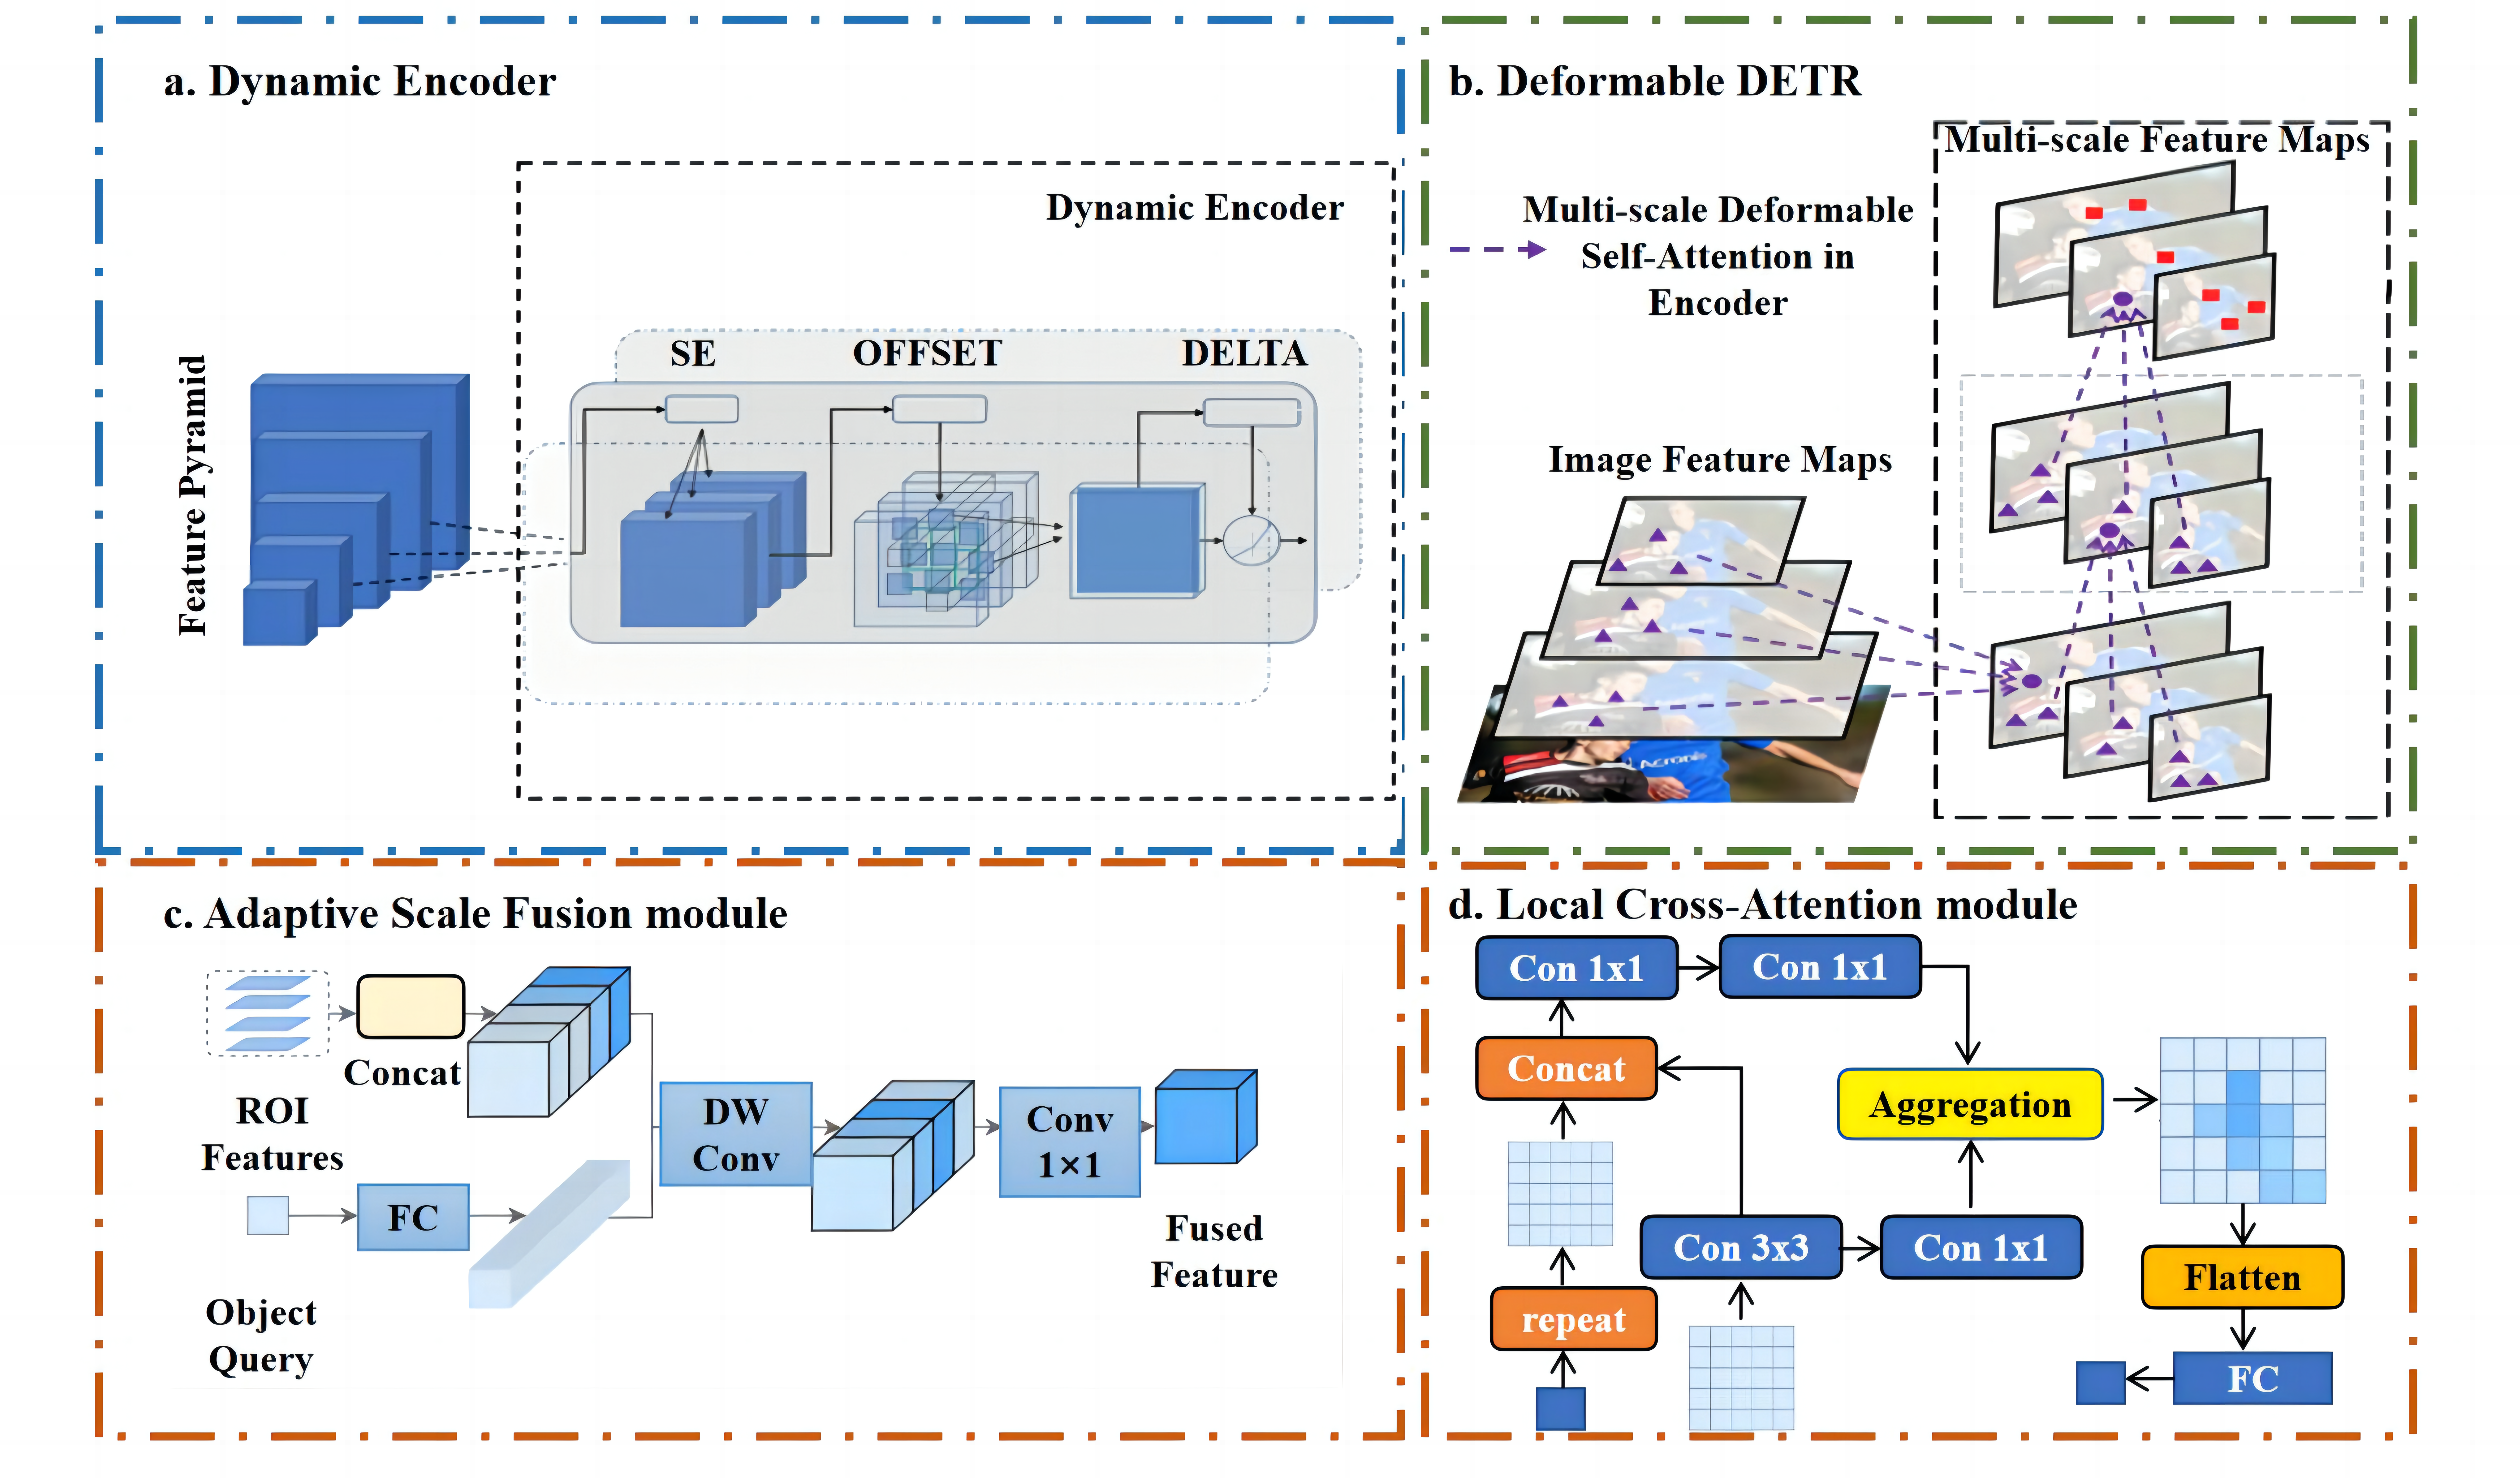
\includegraphics[width=\textwidth]{fig 4}
	\DeclareGraphicsExtensions.
	\caption{Three multi-scale feature methods in small object detection. Figure a employs Deformable Convolution to extract multi-level feature maps. Figure b uses a Convolutional Neural Network as the backbone to extract feature maps of various sizes for multi-scale fusion and employs an attention mechanism to achieve a natural integration of multi-scale features.Figure c and Figure d represent the ASF module and the LCA module in CF-DETR, respectively.}
	\label{fig 1}
\end{figure*}


\subsection{Application of Attention Mechanisms}

The attention mechanism plays a crucial role in small object detection by guiding the model to focus on key areas within an image, significantly enhancing detection performance. This mechanism is primarily implemented through spatial attention, channel attention, or a combination of both. The spatial attention mechanism mimics the human visual system's focus shifts, enabling the model to concentrate on critical parts of the image while ignoring irrelevant regions. This is typically achieved by generating a two-dimensional spatial attention map that weights each position in the input feature map. The advantage of spatial attention lies in its ability to help the model deeply understand local features of the image, which is especially important for small object detection, as small objects may occupy only a tiny portion of the image. Conversely, the channel attention mechanism focuses on the depth dimension of the feature map, i.e., different feature channels. It identifies and enhances the most important feature channels for the current task while suppressing less important ones, allowing the model to concentrate more on critical features. Channel attention is particularly advantageous in dealing with complex backgrounds or subtle differences between target categories. In small object detection, combining these two attention mechanisms allows the simultaneous utilization of spatial and channel information, thereby improving the model's understanding of image content and the accuracy of object detection. As shown in Fig 5, there are two typical algorithms.

ViT and DETR, as the first models to successfully apply attention mechanisms in image classification and object detection tasks, marked a significant milestone for this mechanism in the visual domain. ViT's groundbreaking success revealed the immense potential of attention mechanisms in computer vision and spurred a series of studies exploring how to further optimize and extend Transformers in image processing applications. DETR expanded the application scope of the Transformer architecture in the visual domain. DETR redefined the object detection problem with its innovative set prediction method, using a set-based global loss function and bipartite matching strategy, combined with the Transformer encoder-decoder architecture to directly output predictions in parallel. DETR's design not only improved the efficiency and accuracy of object detection but also opened new possibilities for future research and practice.

To accelerate the convergence of the DETR model, researchers have proposed several improvements. Deformable DETR introduced multi-scale deformable attention modules, which focus on processing critical sampling points in the surrounding area, significantly reducing the number of epochs needed for training and surpassing DETR's performance in small object detection. In contrast, Conditional DETR\cite{meng2021conditional} proposed a conditional spatial query mechanism that enhances localization accuracy and speeds up training through conditional cross-attention. This spatial query carries category and bounding box prediction information extracted from the previous decoder layer, focusing on small areas within the endpoints and target boxes, effectively narrowing the content query range, reducing training difficulty, and accelerating model convergence. Anchor DETR\cite{wang2022anchor} introduced a row-column decoupled attention mechanism, decomposing 2D key features into rows and columns and applying row and column attention respectively, which reduced memory consumption and achieved performance comparable to or better than the standard attention in DETR. These methods optimized the DETR model in various aspects, accelerating convergence speed, and making significant progress in small object detection and memory consumption. Future research can further explore the combination and optimization of these mechanisms to improve model performance and efficiency in a wider range of applications. Despite the introduction of the Transformer architecture, the challenge of small object information loss remains, prompting researchers to propose a series of innovative methods. DeoT\cite{ding2023deot} introduced the E-OTM module, which achieves global feature representation through deformable multi-head self-attention (DMHSA) and is equipped with TBRS, utilizing channel refinement modules (CRM) and spatial refinement modules (SRM) for channel and spatial attention to further refine the output features of the Transformer module. FEA-Swin\cite{xu2022fea} pioneered the foreground-enhanced attention block (FEAB) in the Swin-tiny architecture, strengthening the learning of contextual information and feature distinguishability. Combined with the weighted bidirectional feature pyramid network (BiFPN) and carefully designed skip connections, this method effectively preserved detailed information of small objects. Meanwhile, the BiFPN network optimized the balance between detection accuracy and efficiency by eliminating redundant levels. DKTNet\cite{xu2023dktnet} proposed the Dual-Key Transformer Network (DKTNet), enhancing feature attention through a dual-K enhancement mechanism and replacing traditional spatial-level attention with a channel-level self-attention mechanism to highlight important feature channels and suppress confusing ones. LPSW\cite{xu2021improved} integrated the advantages of Transformer and CNN by designing the locally perceptive Swin Transformer\cite{liu2021swin} backbone network and proposed the Spatial Attention Interlaced Execution Cascade (SAIEC) network framework. Through multi-task learning and an improved spatial attention module, this framework enhanced the network's mask prediction capability and constructed a novel network model using LPSW as the backbone.

These innovative methods provide important insights and practical foundations for addressing the challenge of small object information loss. By introducing global feature representation, foreground-enhanced attention blocks, and dual-key Transformer networks, researchers have made significant progress in the field of small object detection. Future research can further explore the potential and optimization space of these methods to meet the ever-changing demands of practical applications, promoting the development and innovation of small object detection technology.

\begin{figure}[htbp]
	\centering
	\setlength{\abovecaptionskip}{-0.6cm}
	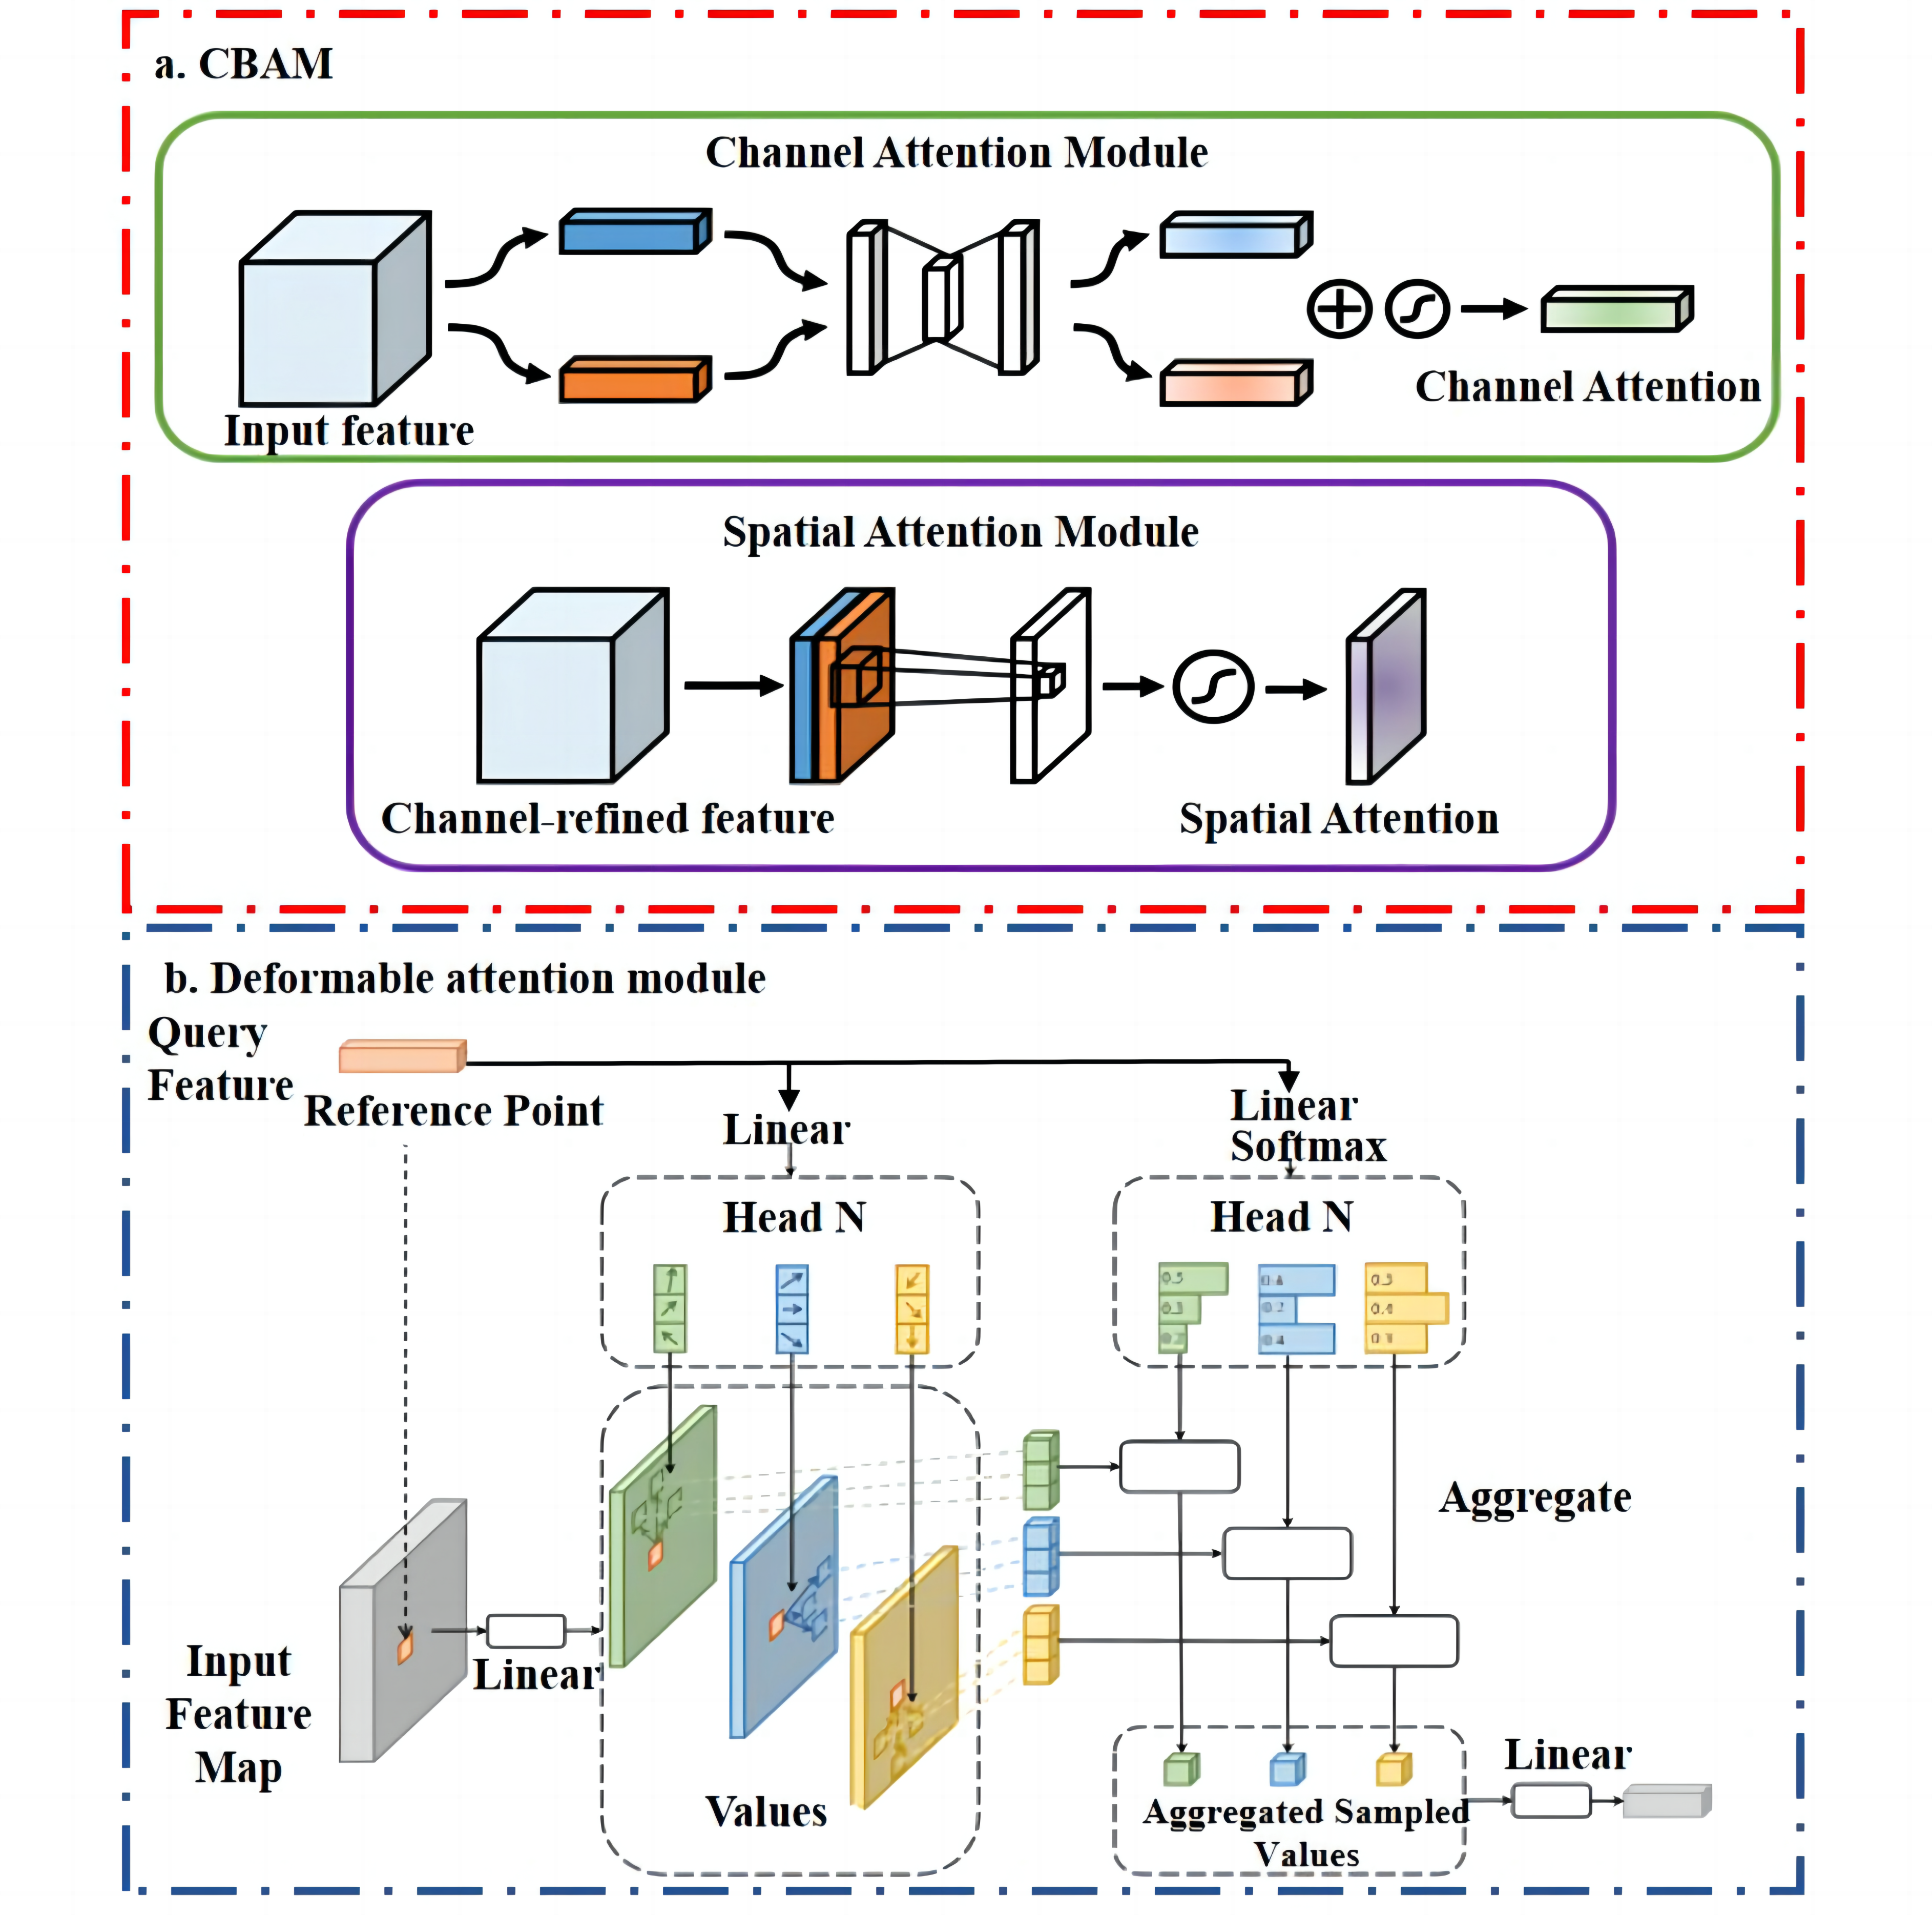
\includegraphics[width=0.5\textwidth]{fig 5}
	\DeclareGraphicsExtensions.
	\caption{Two typical models of attention mechanism application.Figure a combines spatial attention and channel attention to enhance detection accuracy.Figure b adopts deformable attention, allowing the model to dynamically select and focus on the positions with the most informative content.}
	\label{fig 1}
\end{figure}

\subsection{Utilization of Contextual Information}

In the process of detecting small objects, various challenges such as specific scene object detection and occluded targets are often encountered. Due to the limited information contained within small objects, contextual information plays a crucial role in their detection. The application of contextual information ranges from global image-level statistics to local image-level neighboring area information.As shown in Fig 6, there are three typical algorithms.

To enhance the accuracy of small object detection, researchers have explored various strategies for integrating local and global contextual information. CF-DETR\cite{cao2022cf} utilizes its innovative CF decoder layer to combine local and global information, progressively refining features and significantly improving detection accuracy. The Foreground Enhanced Attention Swin Transformer (FEA-Swin) framework and the improved Weighted Bidirectional Feature Pyramid Network (BiFPN) effectively preserve small object details through skip connections. Additionally, researchers have utilized multi-scale feature cascades and attention mechanisms to focus on targets within the image\cite{zeng2022nlfftnet}. IENet\cite{lin2019ienet} combines object appearance and contextual information for robust detection, while the Pyramid Context Learning module (PCL) deeply mines contextual information from different feature levels\cite{zhang2022dino}. These methods optimize feature extraction and processing through multi-scale, multi-level feature integration and attention mechanisms, effectively enhancing the accuracy and robustness of small object detection. This results in more precise detection and identification of small objects, providing new directions and insights for the development of the field.

Considering the limitations of computational resources, researchers are also seeking to reduce over-reliance on context detection techniques in small object detection. Given the diversity of small objects and the complexity of their background information, not all scenarios require contextual techniques. For example, O2DETR\cite{ma2021oriented} posits that global feature interaction is unnecessary for small objects and instead uses depthwise separable convolutions for local interaction to reduce computational load, employing contextual techniques only when there is confusion between the target and background. DyCC-Net\cite{xi2022dycc} dynamically adjusts the network structure to adapt to inputs of varying complexity, achieving efficient input-aware inference, significantly improving inference efficiency, and reducing computational complexity. MATR\cite{sun2022multi} introduced a Selective Context Module (SCM), which features a dynamic selection mechanism to enhance high-resolution features with spatial details, distinguishing them more clearly from noisy backgrounds. DKTNet\cite{xu2023dktnet} suggests that compared to the fully connected computation of traditional Transformer architectures, 2D convolutions can more effectively capture local details and global contextual information, while 1D convolutions can significantly reduce network complexity, providing new directions for optimization. HTDet\cite{chen2023htdet} proposed a new framework based on hybrid transformers, first utilizing a lightweight hybrid transformer network to extract global contextual information, followed by a fine-grained feature pyramid network to address the issue of weak signal disappearance, offering a new solution for small object detection.

These methods collectively emphasize the importance of flexibly adjusting feature extraction strategies based on the requirements of the detection task, to reduce computational complexity and enhance detection accuracy. They provide new directions and insights for the development of small object detection technology, demonstrating how to effectively utilize contextual information in resource-limited scenarios. Future research can build on these foundations to address challenges in practical applications.

\begin{figure*}[htbp]
	\centering
	\setlength{\abovecaptionskip}{-0.6cm}
	\includegraphics[width=\textwidth]{fig 6}
	\DeclareGraphicsExtensions.
	\caption{Three typical methods of context feature processing.[a] O2DETR.[b] MATR.[c] HTDet.}
	\label{fig 1}
\end{figure*}

\subsection{Improvement of Training Strategies}

In the field of deep learning, improving training strategies by adopting diverse methods and techniques optimizes the model training process, thereby enhancing model performance and generalization ability. These strategies encompass auxiliary decoding/encoding techniques, data augmentation, pre-training, and denoising training. This section will detail these strategies and provide a systematic algorithmic classification.As shown in Fig 7, a portion of the algorithms is illustrated.

Auxiliary decoding/encoding is a feedforward network designed for bounding box regression and object classification, enhancing performance by connecting to independent decoding layers. This method trains the model by combining individual losses at different scales, achieving more precise detection results. B. Singh proposed SNIPER\cite{singh2018sniper}, an efficient multi-scale training algorithm for instance-level visual recognition tasks that accelerates the training process by sampling low-resolution regions from a multi-scale image pyramid. To address the scale normalization issue, a Scale-Aware Network (SAN)\cite{kim2018san} maps convolutional features of different scales to a scale-invariant subspace, constructing a unique learning method that considers only inter-channel relationships without spatial information for efficient network learning. N. Bodla's Soft-NMS algorithm\cite{bodla2017soft} avoids object elimination by decaying detection scores of other objects as a continuous function of their overlap with the highest-scoring detection box, applying non-maximum suppression in post-processing. Due to the network's general lack of robustness to scale variations, B. Singh also proposed a detector that trains and tests at the same scale on the image pyramid\cite{singh2018analysis}, using a scale-normalized training scheme that only trains on objects within the desired scale range. To better extract features at various scales, VIDT\cite{song2021vidt} combined multi-layer deformable Transformer decoders, generating new [DET] tokens through multi-scale deformable attention to aggregate critical content from multi-scale feature maps, improving detection performance. TTRD\cite{li2022transformer} aims to aggregate features of multi-scale global spatial positions and simulate interactions between paired instances through a modified Transformer. To reduce computational resource consumption, MDef-DETR\cite{maaz2021multi} applied multi-scale hierarchical modeling with visual priors in a pure Transformer architecture. As the model deepens, feature resolution decreases while the number of channels increases, effectively reducing Transformer computational resources. CBNet\cite{liang2022cbnet} proposed a feature fusion technique where the output features of the previous backbone network (i.e., high-level features) are used as part of the input features for subsequent backbone networks, progressively expanding the receptive field. This iterative feature transmission method helps capture and utilize multi-scale information at different stages for more effective small object detection.

Data augmentation is a technique to expand the dataset through various methods without substantially increasing data, which becomes an effective solution given the scarcity of small object datasets. This technique enriches the detection dataset by applying multiple augmentation techniques such as rotation, flipping, scaling, cropping, translation, and adding noise. Supervised data augmentation methods include SMOTE\cite{chawla2002smote}, SamplePairing\cite{inoue2018data}, and mixup\cite{chawla2002smote}, while unsupervised methods include GAN\cite{aggarwal2021generative} and AutoAugment\cite{cubuk2018autoaugment}. Sw-YoloX\cite{ding2023sw} augments training data by randomly scaling, cropping, and arranging four images into one, then generating new training samples by mixing two images, enhancing the model's generalization ability. NLFFTNet\cite{zeng2022nlfftnet} introduced a configurable hybrid splicing dynamic data augmentation method to address data imbalance between different categories. To avoid overfitting, T-TRD  combined data augmentation with Transformers to improve the detection performance of remote sensing images.

Pre-trained models are an application of transfer learning that learns context-aware representations of each member from large datasets. Pre-trained models can transfer knowledge learned from open domains to downstream tasks to improve the performance of low-resource tasks. Due to significant differences between source datasets (e.g., ImageNet) and target datasets (i.e., remote sensing image datasets), TRD proposed an attention mechanism-based transfer CNN (T-TRD) to adapt pre-trained models for better remote sensing image object detection. FP-DETR\cite{wang2021fp} explored how to fully pre-train an encoder-only transformer and smoothly fine-tune it for object detection through task adapters. Building on this, Group DETR v2\cite{chen2022group} further improved performance through encoder-decoder pre-training and fine-tuning.

Denoising training introduces noise during the training process and trains the model to reconstruct or predict the original data without noise. This method can improve the model's generalization ability by forcing the model to learn to extract and recover useful information from noisy data. In object detection, particularly in training Detection Transformer (DETR) models, denoising training addresses the issue of slow model convergence. DINO\cite{zhang2022dino} improved the performance and efficiency of previous DETR models by using contrastive denoising training, a mixed query selection method for anchor initialization, and a two-stage look-ahead scheme for box prediction. DN-DETR\cite{li2022dn} proposed a novel denoising training method to accelerate DETR training. In addition to the Hungarian loss, their method inputs noisy ground truth bounding boxes into the Transformer decoder and trains the model to reconstruct the original boxes, effectively reducing the difficulty of bipartite matching and speeding up convergence.

These innovative training strategy improvements bring new possibilities to the field of small object detection, enabling models to learn more effectively from complex data and enhance their recognition accuracy. Future research is expected to further optimize algorithms using these strategies, reduce computational costs, and improve application capabilities in various real-world environments, especially in resource-constrained scenarios. This will drive advancements in small object detection technology in critical areas such as autonomous driving, remote sensing image analysis, and medical imaging diagnosis, providing powerful technical support for solving complex real-world problems.

\begin{figure*}[htbp]
	\centering
	\setlength{\abovecaptionskip}{-0.6cm}
	\includegraphics[width=\textwidth]{fig 7}
	\DeclareGraphicsExtensions.
	\caption{Three typical methods of improving training strategies.[a] FP-DETR.[b] DN-DETR.[c] T-TRD.}
	\label{fig 1}
\end{figure*}


\subsection{Exploitation of Spatio-Temporal Information}

The utilization of spatiotemporal information refers to leveraging the spatial and temporal relationships of targets across consecutive frames or scenes to enhance detection accuracy. This strategy is particularly applicable to video or dynamic environments. Early methods for small object detection in videos, such as R-CNN, relied on Region Proposal Networks (RPN) to generate candidate regions and combined them with deep learning feature extraction to improve classification accuracy. However, these methods were slow and involved complex post-processing. Improvements like Fast R-CNN and Faster R-CNN optimized the algorithm structure to increase detection speed. Models like SSD and YOLO accelerated detection by using single-shot detection on multi-scale feature maps and framing detection as a regression problem, though at the cost of some accuracy. The TPN\cite{zhu2021tph} model enhanced video object detection performance by integrating target feature representations through video pipeline proposals, but this increased computational resource demands.

Traditional Video Object Detection (VOD) methods depended on multi-stage processes and manually designed feature aggregation components, such as optical flow models and relational networks, leading to inefficiencies. TransVOD\cite{zhou2022transvod} introduced a spatiotemporal Transformer architecture, simplifying the VOD process, reducing model complexity and computational costs, and improving detection accuracy and efficiency by establishing long-term dependencies across video frames. Aerial Trans\cite{liu2021aerial} addressed issues of occlusion, loss, and drift in small object tracking by proposing two trackers that utilize Transformer attention mechanisms to supplement small object contextual information, enhancing tracking performance.As shown in fig 8, SparseVOD\cite{hashmi2022spatio} proposed an innovative video object detection process that uses Sparse R-CNN to generate detection objects by incorporating temporal information, alleviating the burden of post-processing and enabling end-to-end training. PTSEFormer\cite{wang2022ptseformer} introduced a new detection method that incrementally incorporates temporal and spatial information to enhance features rather than aggregating them all at once, more effectively utilizing contextual information from adjacent frames. This method uses the Transformer-based detector DETR, avoiding heavy post-processing. VSTAMcite{fujitake2022video} presented a sparse aggregation per-element feature method to reduce processing time and memory costs, enhancing features per element before object candidate region detection to improve accuracy. This approach maintains high accuracy while reducing computational and memory demands. FAQ\cite{cui2023faq} addressed the issue of feature degradation in video object detection by proposing a method that utilizes temporal information from adjacent frames and merges their features, demonstrating its effectiveness.

These methods leveraging spatiotemporal information bring unprecedented depth and dimension to small object detection, making recognition and tracking in dynamic environments more precise and reliable. Future research may focus on further refining and optimizing these methods for seamless integration and efficient operation in a broader range of application scenarios.

\begin{figure*}[htbp]
	\centering
	\setlength{\abovecaptionskip}{-0.6cm}
	\includegraphics[width=\textwidth]{fig 8}
	\DeclareGraphicsExtensions.
	\caption{Three typical methods of utilizing spatiotemporal information.Figure A simplifies the process by introducing a spatial-temporal Transformer architecture. Figure B proposes two types of small target trackers to provide a global response. Figure C presents an innovative video object detection workflow, using Sparse R-CNN combined with temporal information to generate detection objects. }
	\label{fig 1}
\end{figure*}

\subsection{Efficiency and Optimization in Computing}

In the classification of small object detection algorithms, computational efficiency and optimization constitute a crucial research area. This field focuses on reducing the computational resources required during algorithm execution while maintaining or enhancing detection performance. The primary objective is to develop algorithms capable of processing large volumes of image data quickly and accurately, particularly in resource-constrained environments such as mobile devices or edge computing platforms.

Traditional Transformer models, due to their use of global self-attention, consume significant computational resources when processing large images. Deformable DETR addresses this issue by introducing a deformable attention mechanism that calculates attention only at a sparse set of positions in the image, effectively reducing computational complexity and accelerating model convergence. Swin Transformer adopts a hierarchical feature map that progressively reduces in size with network depth, similar to traditional CNNs, which helps capture features from coarse to fine granularity while improving efficiency. Swin Transformer significantly reduces computation by performing self-attention calculations within local windows.

As shown in fig 9,O2DETR\cite{ma2021oriented} suggests that global feature interaction is unnecessary and employs depthwise separable convolutions for local interactions, further reducing computation and speeding up model convergence. Conditional DETR\cite{meng2021conditional} reduces training difficulty by learning conditional spatial queries for decoder multi-head cross-attention, narrowing the spatial range of content queries. DAB-DETR\cite{liu2022dab} accelerates training convergence by directly using box coordinates as queries for the Transformer decoder and dynamically updating them layer by layer, leveraging positional priors to enhance feature similarity. QueryDet\cite{yang2022querydet} introduces a Cascaded Sparse Query (CSQ) mechanism that efficiently utilizes high-resolution features by first obtaining the rough location of small objects on high-level feature maps and then conducting detailed queries on low-level feature maps, thereby improving small object detection performance while maintaining fast inference speed.

These advanced methods for computational efficiency and optimization in the field of small object detection not only demonstrate technological innovation but also lay a solid foundation for achieving efficient and precise small object detection in various application scenarios. Future research can further explore the potential of these methods, integrating additional optimization techniques and innovative algorithms to meet the demands of different applications. Particularly in resource-constrained environments like mobile devices and edge computing platforms, these efficient small object detection algorithms will play a crucial role.

\begin{figure*}[htbp]
	\centering
	\setlength{\abovecaptionskip}{-0.6cm}
	\includegraphics[width=\textwidth]{fig 9}
	\DeclareGraphicsExtensions.
	\caption{Four typical methods of optimizing computational efficiency.}
	\label{fig 1}
\end{figure*}

\section{Datasets}

Datasets are the foundation of small object detection and an important basis for evaluating the performance of small object detection methods. Different datasets have distinct characteristics and application scenarios, posing varying requirements and challenges for small object detection methods. Therefore, selecting appropriate datasets is crucial for the research and application of small object detection.As shown in table 2, this section will provide an overview of some publicly available datasets for specific scenarios, introducing their sources, content, scale, and features. It will also compare their difficulty levels and applicability, as well as quantitatively and qualitatively assess and analyze the performance of various small object detection methods on different scenario datasets. This will help determine the most effective small object detection methods for that scenario.

% Table generated by Excel2LaTeX from sheet 'Sheet1'
% Table generated by Excel2LaTeX from sheet 'Sheet1'
\begin{table*}[htbp]
	\centering
	\caption{Summary of Datasets}
	\resizebox{\textwidth}{!}{  % Resize table to fit the page width
		\setlength{\tabcolsep}{5pt}  % Adjust column spacing
		\renewcommand{\arraystretch}{1.5}  % Adjust row spacing
		\begin{tabular}{
				>{\centering\arraybackslash}p{9.125em}
				>{\centering\arraybackslash}p{2cm}
				>{\centering\arraybackslash}p{3cm}
				>{\centering\arraybackslash}p{3cm}
				>{\centering\arraybackslash}p{3cm}
				>{\centering\arraybackslash}p{4cm}}
			\toprule
			Dataset & Years & Object Classes & Instances & Country & Application \\
			\midrule
			MS COCO & 2015 & 91 & 2,500,000 & United States & \multirow{4}{*}{Generic Applications} \\
			PASCAL VOC & 2012 & 20 & 27,450 & United Kingdom & \\
			WIDER FACE & 2016 & 61 & 393,703 & China & \\
			SKU-110K & 2019 & 110,712 & 147.4 per image & The State of Israel & \\
			\midrule
			DAIR-V2X & 2021 & 10 & - & China & \multirow{5}{*}{Self-Driving} \\
			Argoverse & 2020 & 15 & 11,052 & United States & \\
			KAIST Multispectral Pedestrian & 2015 & 4 & - & Korea & \\
			CQCAR-20 & 2024 & 20 & 11,000 & China & \\
			Cityscapes & 2016 & 30 & - & Germany & \\
			\midrule
			DOTA & 2017 & 15 & 188,282 & China & \multirow{4}{*}{Aerial Images} \\
			HRSC2016 & 2016 & 27 & 2,976 & China & \\
			UCAS-AOD & 2014 & 2 & 18,895 & China & \\
			UAV123 & 2016 & - & - & Saudi Arabia & \\
			\midrule
			AMMW & 2024 & 30 & - & China & \multirow{4}{*}{Active Milli-Meter Wave Images} \\
			MM-Fi & 2023 & 40 & - & Singapore & \\
			nuScenes & 2019 & 23 & - & Singapore & \\
			RadarScenes & 2016 & 5 & - & Germany & \\
			\bottomrule
	\end{tabular}}
	\label{tab:addlabel}
\end{table*}





\subsection{General image datasets}

General image datasets refer to collections of images that encompass a wide variety of categories and scenes, typically used to assess the universality and robustness of object detection methods. In these datasets, small objects are usually defined as targets that occupy a small proportion or resolution in the image, such as pedestrians, vehicles, animals, etc.As shown in fig 10, the following are commonly used general image datasets:

MS COCO: Microsoft Common Objects in Context (MS COCO) is a large-scale dataset built by Microsoft for object detection, segmentation, keypoint detection, and image captioning. It contains 91 categories, 328,000 images, and 2,500,000 object instances. Small objects in this dataset are defined as targets with bounding box sizes smaller than 32×32 pixels, accounting for 23.5\% of all objects. 

PASCAL VOC: PASCAL Visual Object Classes (PASCAL VOC) is a dataset created by the computer vision group at the Technical University of Munich, Germany, for object detection, segmentation, classification, and action recognition. It includes 20 categories, 11,540 images, and 27,450 object instances. Small objects in this dataset are generally defined as targets where the width and height of the bounding box are less than 10\% of the image’s width and height, accounting for 14.8\% of all objects. 

WIDER FACE\cite{yang2016wider}: WIDER FACE is a dataset for face detection released by researchers at the Hong Kong University of Science and Technology in 2018. It includes 61 categories, 32,203 images, and 393,703 face instances. Small objects in this dataset are generally defined as faces with bounding box areas smaller than 1024 pixels, accounting for 29.7\% of all faces.

SKU-110K\cite{goldman2019precise}: The SKU-110K dataset is a dense collection of retail shelf images intended to support research in object detection tasks. Developed by Eran Goldman et al., it contains over 110,000 unique Stock Keeping Unit (SKU) categories. The objects in these categories are densely arranged, often appearing similar or even identical, and are positioned very close to each other. The SKU-110K dataset includes 11,762 images taken in dense scenes, with over 1.7 million bounding box annotations, totaling approximately 1,733,678 instances. These images are collected from thousands of supermarkets, featuring varying scales, perspectives, lighting conditions, and noise levels. All images are adjusted to a resolution of one million pixels.

The advantage of these datasets lies in the diversity of categories and scenes, which helps demonstrate the universality and robustness of small object detection. However, they also have disadvantages: the number and proportion of small objects are low, leading to sample imbalance and difficulty in fully training and evaluating small object detection methods. Additionally, since the definition of small objects varies across different datasets, cross-dataset performance comparison is challenging.

Considering these characteristics and limitations of general image datasets, there are several key aspects to focus on for future research and applications. Firstly, developing datasets containing more small object samples or using synthetic augmentation techniques to balance datasets will be an important research direction to address the issue of low quantity and proportion of small objects. Secondly, unifying or standardizing the definition of small objects will help achieve fairer and more consistent performance evaluations across different datasets. Lastly, as general image datasets cover a rich variety of categories and scenes, they provide researchers with valuable opportunities to explore and test the generalization capabilities of object detection methods and their adaptability to different environments. In summary, general image datasets play a crucial role in the research and application of small object detection, and in-depth study and optimization of these datasets will have a profound impact on advancing the technology in this field.

\begin{figure*}[htbp]
	\centering
	\setlength{\abovecaptionskip}{-0.6cm}
	\includegraphics[width=\textwidth]{fig 10}
	\DeclareGraphicsExtensions.
	\caption{Examples of detection results on Generic Applications Dataset.}
	\label{fig 1}
\end{figure*}

\subsection{Datasets for Intelligent Vehicles}

Datasets for intelligent vehicles are large-scale collections specifically designed for intelligent vehicle technologies, such as autonomous driving and vehicle perception systems. These datasets typically contain a vast amount of images, videos, sensor data, and other types of information collected from real-world scenarios, used to train and test intelligent vehicle algorithms. As shown in fig 11,the following are commonly used datasets in the field of intelligent vehicles:

DAIR-V2X\cite{yu2022dair}: DAIR-V2X (Vehicle-to-Everything Autonomous Driving Dataset) is released jointly by Tsinghua University’s Institute for AI Industry Research (AIR), Beijing High-level Autonomous Driving Demonstration Area, Beijing CarNet Technology Development Co., Baidu Apollo, and Beijing Academy of Artificial Intelligence. It is the world’s first large-scale, multimodal, multi-view dataset for vehicle-to-everything autonomous driving research. It contains a series of data based on real autonomous driving scenarios, aimed at promoting smarter decision-making and enhancing the safety of autonomous driving. The dataset allows the simultaneous use of infrastructure and vehicle-end information to track and predict the behavior of surrounding traffic participants. Specifically, the DAIR-V2X dataset includes the following parts:
DAIR-V2X-C (Collaborative Dataset): Contains 38,845 frames of image data and 38,845 frames of point cloud data for studying vehicle-to-everything autonomous driving. These data are collected from real scenarios and include both 2D and 3D annotations.
DAIR-V2X-I (Infrastructure Dataset): Contains 10,084 frames of image data and 10,084 frames of point cloud data, focusing more on roadside monocular 3D object detection tasks.
DAIR-V2X-V (Vehicle-end Dataset): Contains 22,325 frames of image data and 22,325 frames of point cloud data for studying vehicle-end perception and prediction. These datasets achieve vehicle-to-everything spatio-temporal synchronized annotation for the first time, with a rich variety of sensor types, including vehicle-end cameras, vehicle-end LiDAR, roadside cameras, and roadside LiDAR. The 3D annotation attributes of obstacle targets are comprehensive, annotating 10 types of common road obstacle targets.

Argoverse\cite{chang2019argoverse}: The Argoverse dataset is released by Argo AI, Carnegie Mellon University, and Georgia Institute of Technology, containing two parts: 3D Tracking and Motion Forecasting. Argoverse is somewhat different from Waymo; although it also includes LiDAR and camera data, it only covers 113 scenes recorded in Miami and Pittsburgh. Its uniqueness lies in being the first dataset to include high-definition map data, mainly featuring 290 kilometers of lane maps in Pittsburgh and Miami, with information such as location, connections, traffic signals, elevation, etc. Its sensors consist of 2 LiDARs, 7 high-resolution ring cameras (1920 × 1200), and 2 stereo cameras (2056 × 2464). In Argoverse 3D tracking, it includes 3D tracking annotations for 113 scenes, each segment lasting 15-30 seconds, totaling 11,052 tracked objects, annotating objects within 5 meters, with 15 labels, 70\% of which are vehicles, and 30\% pedestrians, bicycles, motorcycles, etc. In Argoverse Motion Forecasting, it includes 324,557 scenes, each lasting 5 seconds, and contains a 2D bird’s-eye view of each tracked object sampled at 10 Hz.

KAIST Multispectral Pedestrian\cite{hwang2015multispectral}: The KAIST Multispectral Pedestrian dataset is released by the Korea Advanced Institute of Science and Technology, providing a multispectral pedestrian detection dataset with color-thermal image pairs during day and night. The dataset improves the accuracy of pedestrian detection by complementing the advantages of color images and thermal imaging, overcoming previous issues such as pedestrian occlusion, cluttered backgrounds, and unclear nighttime imaging. It provides 95,328 pairs of color-thermal images during day and night, aligning images through a beam splitter to eliminate image parallax. The data is collected in Seoul, South Korea, with an image resolution of 640x480, 103,128 manual 2D box annotations, 1,182 pedestrians, and four different types of annotations: person, people (unclear human figures), cyclist, person? (uncertain if a pedestrian).

Cityscapes\cite{cordts2016cityscapes}: Cityscapes is released by the Mercedes-Benz Research and Development Center and is recognized as one of the most authoritative and professional semantic segmentation evaluation sets in the field of autonomous driving. The dataset collects urban scenes from 50 cities in Germany and neighboring countries across three seasons: spring, summer, and autumn, and captures stereoscopic vision video sequences using binocular cameras. After conversion, this dataset can be used for object detection tasks, providing 2,975 and 500 data for model training and validation, respectively. It includes categories such as people, riders, cars, trucks, buses, trains, motorcycles, and bicycles, totaling 30.

CQCAR-20:As shown in fig 12, this dataset is meticulously produced by the Safety-AI lab team at Chongqing University, with materials sourced from road traffic scenes in Chongqing City. The dataset is specifically designed for traffic road object detection in the intelligent vehicle field, covering nearly 20 categories, including but not limited to traffic lights, traffic signs, pedestrians, and bicycles, which we consider to fall within the category of small objects. In terms of quantity, the dataset contains about 3,000 training set images, 500 validation set images, and 500 test set images, with approximately 11,000 target boxes annotated in total. By providing such a specialized dataset, the Safety-AI lab at Chongqing University aims to support researchers in the field of intelligent vehicles, especially those teams dedicated to training and detection in small object scenarios, thereby enhancing the perception and response capabilities of intelligent vehicle systems in real road environments.

\begin{figure*}[htbp]
	\centering
	\setlength{\abovecaptionskip}{-0.6cm}
	\includegraphics[width=\textwidth]{fig 11}
	\DeclareGraphicsExtensions.
	\caption{Examples of detection results on intelligent Vehicle Domain Datasets.}
	\label{fig 1}
\end{figure*}


\begin{figure*}[htbp]
	\centering
	\setlength{\abovecaptionskip}{-0.6cm}
	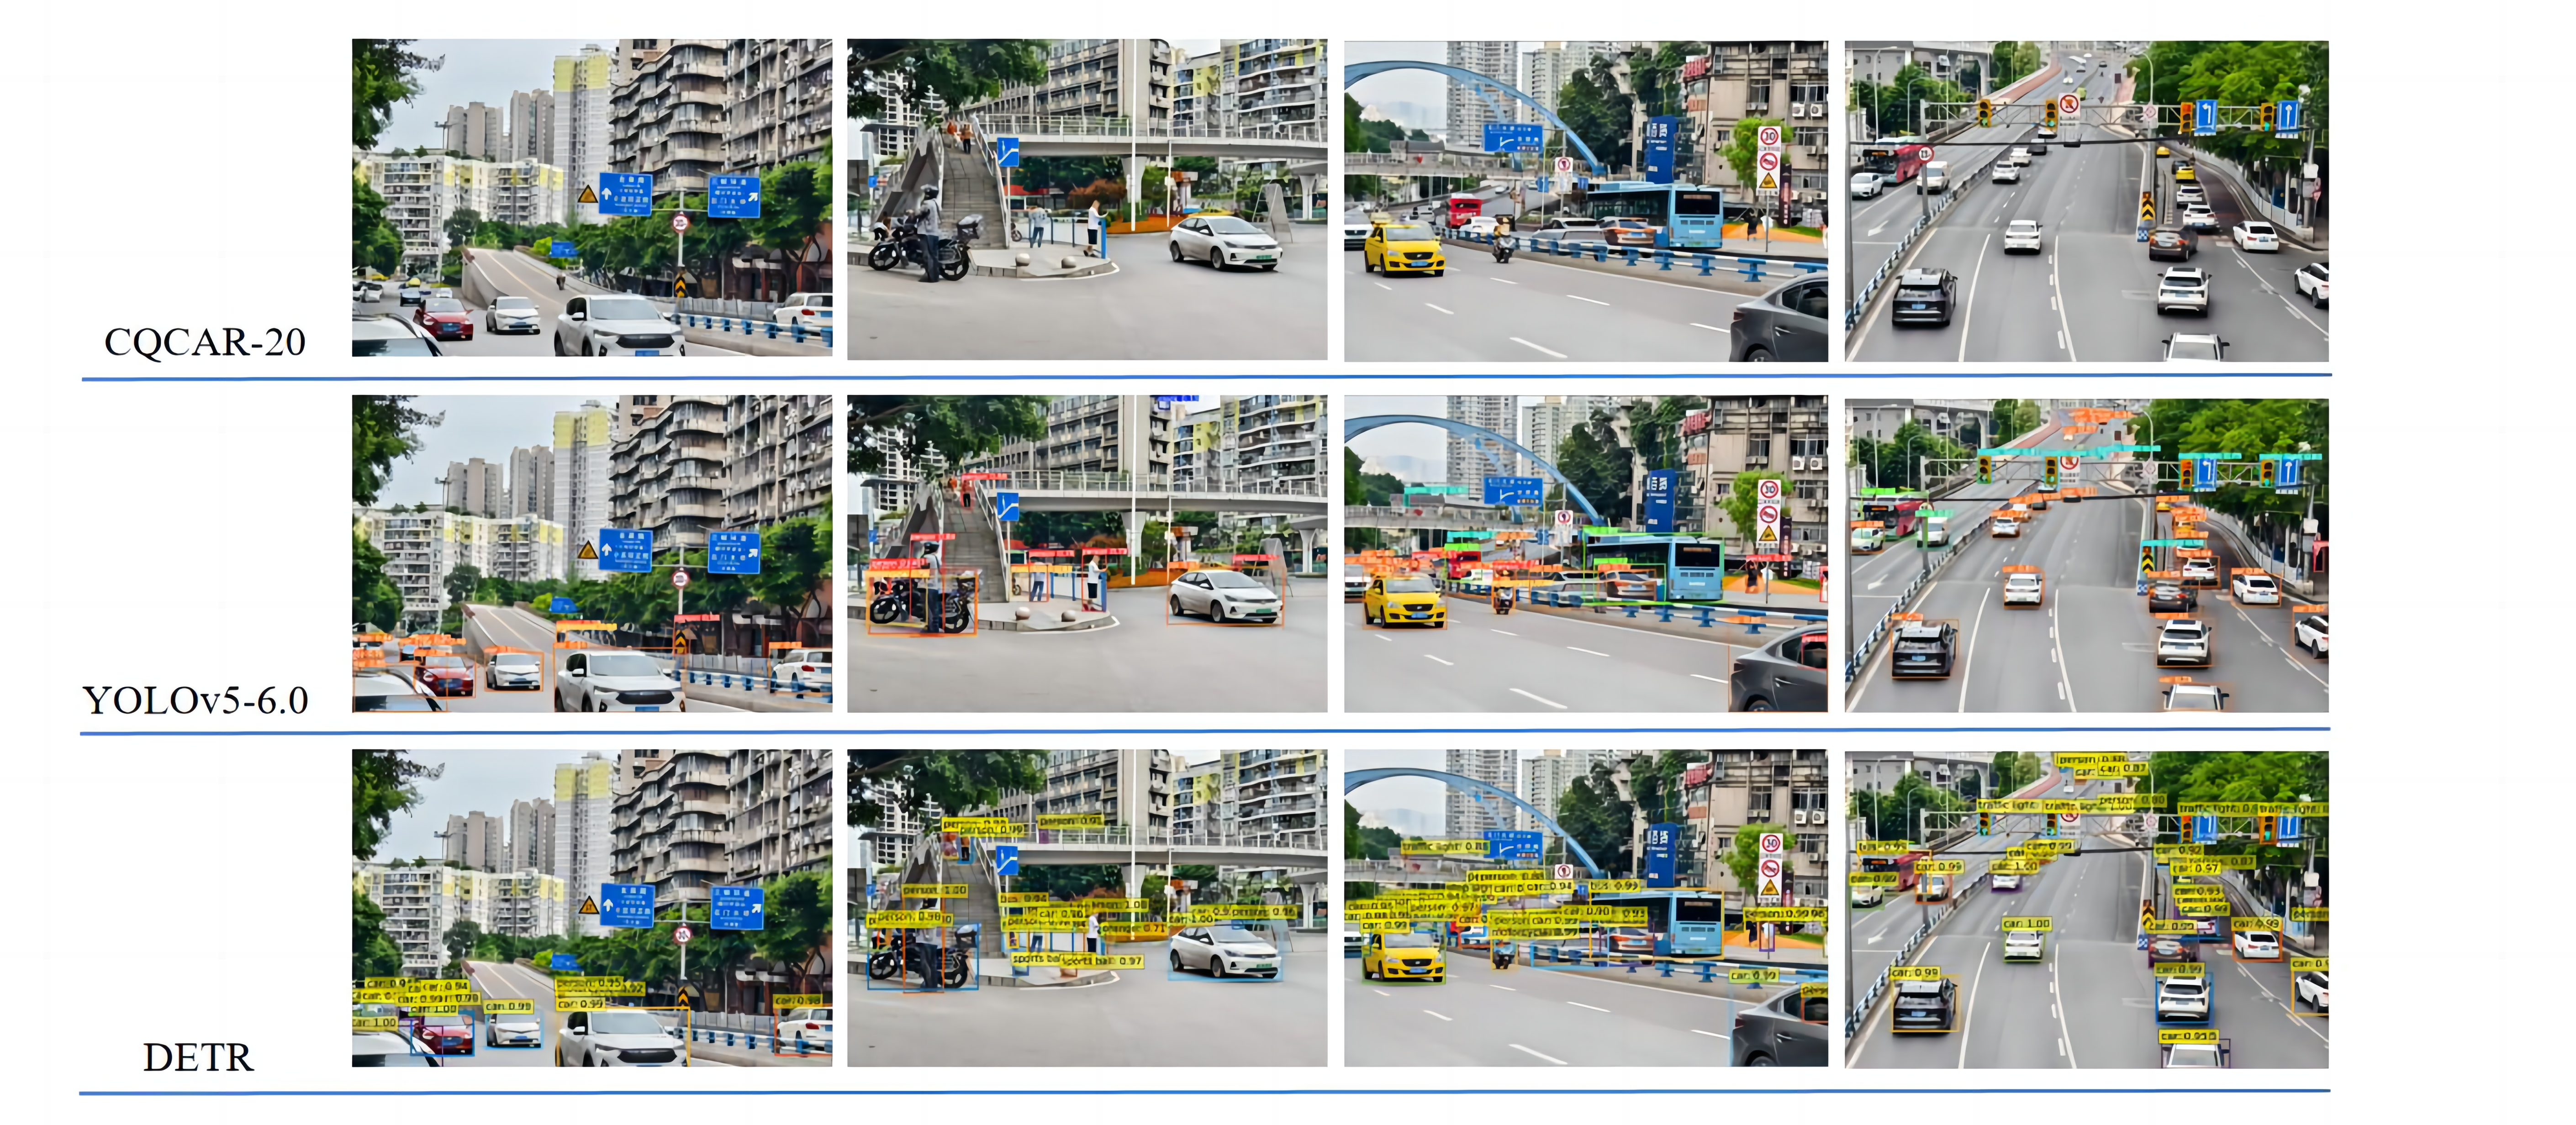
\includegraphics[width=\textwidth]{fig 12}
	\DeclareGraphicsExtensions.
	\caption{Examples of detection results on CQCAR-20 dataset for YOLOv5 based on CNN and DETR based on Transformer.}
	\label{fig 1}
\end{figure*}

\subsection{Aerial Image Datasets}

Aerial image datasets, collections of images captured from a high-altitude perspective, are commonly used to evaluate object detection methods in the field of remote sensing. In these datasets, small objects refer to entities that appear as tiny in size or low in resolution in the images, such as vehicles, ships, and airplanes. As shown in fig 13,there are some of the main aerial image datasets:

DOTA\cite{xia2018dota}: DOTA (A Large-scale Dataset for Object Detection in Aerial Images) is a large-scale dataset for object detection in aerial images, containing 15 categories, 2,806 images, and 188,282 object instances. Small objects in this dataset are defined as targets with both width and height less than 30 pixels, accounting for 13.7\% of all objects. The evaluation metric for this dataset is mean Average Precision (mAP), calculated at an IoU threshold of 0.5.

HRSC2016\cite{liu2017high}: HRSC2016 (High Resolution Satellite Image Ship Detection Dataset) is a dataset for ship detection in aerial images, containing 27 categories, 1,061 images, and 2,976 ship instances. Small objects in this dataset are defined as ships with both width and height less than 20 pixels, accounting for 10.8\% of all ships. The evaluation metric for this dataset is mAP, calculated at an IoU threshold of 0.5.
UCAS-AOD\cite{zhu2015orientation}: UCAS-AOD (University of Chinese Academy of Sciences Aerial Object Detection) is a dataset for object detection in aerial images, containing 2 categories, 910 images, and 18,895 object instances. Small objects in this dataset are defined as targets with both width and height less than 16 pixels, accounting for 11.2\% of all objects. The evaluation metric for this dataset is mAP, calculated at an IoU threshold of 0.5.

UAV123\cite{mueller2016benchmark}: This dataset contains 123 videos captured by drones, one of the largest object tracking datasets with over 110K frames. These videos are shot by drones at low altitudes, and each video comes with corresponding ground truth annotations.

The notable advantages of these aerial image datasets are that they provide high-resolution images and a rich variety of target types, effectively demonstrating the practical application potential of small object detection in the field of remote sensing. However, they also have clear limitations: the singularity of categories and simplicity of scenes limit the assessment of the generalization ability and robustness of small object detection methods. Additionally, due to the lack of uniformity in the definition of small objects, performance comparisons between these datasets are also constrained. In aerial images, objects appear particularly small due to their relative distance from the camera, and the bird’s-eye view perspective means that objects can appear anywhere in the image, bringing additional challenges to the object detection task.

When evaluating the performance of different algorithms in such application scenarios, we have chosen the DOTAcite{xia2018dota} dataset as the testing benchmark because it has become a widely applied standard in the field of object detection. Among CNN-based methods, ReDet\cite{han2021redet} has shown excellent performance, especially in terms of rotational invariance. This method uses a rotation-equivariant network and a rotation-invariant RoI alignment mechanism to extract features and accurately predict the orientation and position of targets. With data augmentation techniques such as multi-scale training, testing, random rotation cropping, and random rotation flipping, ReDet has improved the model’s robustness in detecting small objects and multi-directional targets. In a hybrid framework, ReDet achieves the highest accuracy value (80.89\%) with only 12 training epochs, thanks to its multi-scale learning strategy and pre-training on the ImageNet dataset.

\begin{figure*}[htbp]
	\centering
	\setlength{\abovecaptionskip}{-0.6cm}
	\includegraphics[width=\textwidth]{fig 13}
	\DeclareGraphicsExtensions.
	\caption{Examples of detection results on Aerial Image Dataset.}
	\label{fig 1}
\end{figure*}

\subsection{Active Millimeter Wave Datasets}

Active Millimeter Wave (AMMW) datasets,as shown in fig 14,typically composed of data collected using active millimeter-wave radar sensors, are crucial resources for evaluating object detection methods in scenarios that require privacy protection, adaptation to harsh weather, and low-light conditions. In these datasets, small objects generally refer to those that produce weak reflections in radar signals or have a low signal-to-noise ratio, such as human bodies, metal items, and animals. Here are some of the primary active millimeter-wave datasets:

AMMW\cite{yu2021active}: AMMW (Active Millimeter Wave) is a dataset for active millimeter-wave imaging, containing two subsets: AMMW-A and AMMW-B. AMMW-A includes 58k single-channel millimeter-wave images taken from different angles, each with a human subject possibly carrying one or more concealed items. AMMW-B consists of 2k three-dimensional millimeter-wave images taken from the front and back, each with a human subject possibly carrying one or more concealed items. Small objects in this dataset are defined as targets with both width and height less than 20 pixels, accounting for 12.4\% of all objects. The evaluation metrics for this dataset are Detection Rate (DR) and False Alarm Rate (FAR), calculated at different confidence thresholds.

MM-Fi\cite{yang2024mm}: MM-Fi (Multi-Modal Non-Intrusive 4D Human Dataset for Versatile Sensing) is a dataset for multi-modal non-intrusive human perception, containing 320,000 synchronized frames of 40 human subjects across 5 modalities (active millimeter-wave radar, RGB camera, depth camera, thermal imager, and IMU). Small objects in this dataset are defined as targets with both width and height less than 10 pixels, accounting for 9.6\% of all objects. The evaluation metric for this dataset is mean Average Precision (mAP), calculated at different IoU thresholds (0.5, 0.75, 0.5:0.95).

nuScenes\cite{caesar2020nuscenes}: nuScenes (A multimodal dataset for autonomous driving) is a multi-modal dataset for autonomous driving, containing 1.4 million images (from 6 cameras), 390,000 frames of LiDAR data (from 1 LiDAR), 1.4 million frames of millimeter-wave radar data (from 5 radars), and 1.4 million object annotations in 40,000 keyframes collected from 1,000 driving scenes in Boston and Singapore. Small objects in this dataset are defined as targets with both width and height less than 32 pixels, accounting for 15.2\% of all objects. The evaluation metric for this dataset is mAP, calculated at different scales (small, medium, large) and IoU thresholds (0.5, 0.75, 0.5:0.95).

RadarScenes\cite{schumann2021radarscenes}: RadarScenes (A Real-World Radar Point Cloud Data Set for Automotive Applications) is a real-world radar point cloud dataset for automotive applications, containing data from 10 scenes collected by 4 77GHz autonomous driving radar sensors and 1 documentary camera, including various road conditions in urban, rural, and highway settings. Small objects in this dataset are defined as targets with both width and height less than 20 pixels, accounting for 12.4\% of all objects. The evaluation metric for this dataset is mAP, calculated at an IoU threshold of 0.5.

The AMMW datasets, with their multi-modal data and complex scenarios, fully demonstrate the application potential and challenges faced by active millimeter-wave radar in various perception tasks. However, these datasets are limited by their relatively small data volume and limited annotation information, insufficient to support the full training and evaluation of deep learning algorithms. Additionally, due to the lack of uniformity in the definition of small objects, performance comparisons between different datasets are challenging. In our research, we chose the AMMW dataset for experimentation, as it is currently the largest-scale active millimeter-wave imaging dataset, offering a wealth of data and diversity conducive to testing the generalization ability and robustness of small object detection algorithms.

Our research focuses on two types of methods: one based on CNN algorithms and the other on hybrid architectures combining CNN and Transformer. Among CNN methods, Yolov5 stands out, combining techniques such as anchor box adaptation, multi-scale prediction, label smoothing, and multi-modal fusion to effectively adapt to the detection needs of small and irregular objects and handle the noise and blurry millimeter-wave images in the AMMW dataset. At the same time, Yolov5 leverages the advantages of multi-view millimeter-wave images to improve detection accuracy and efficiency. In hybrid architectures, the MATR algorithm performs excellently, enhancing the perception and localization accuracy of small objects through multi-head self-attention mechanisms and multi-scale feature fusion. MATR’s multi-head self-attention mechanism captures global dependencies between targets of different scales and orientations, thus enhancing the detection capability for irregular targets in the AMMW dataset. Additionally, MATR employs anchor box adaptation and multi-modal fusion techniques to adapt to the characteristics of small and irregular targets in the AMMW dataset, further improving detection accuracy and efficiency.

\begin{figure*}[htbp]
	\centering
	\setlength{\abovecaptionskip}{-0.6cm}
	\includegraphics[width=\textwidth]{fig 14}
	\DeclareGraphicsExtensions.
	\caption{Examples of detection results on Aerial Image Dataset.}
	\label{fig 1}
\end{figure*}

\subsection{Summary and Analysis of Datasets}

In the analysis of current datasets for small object detection, several key characteristics can be identified. Firstly, there is a disparity in the definition of small objects; some are based on the size of the bounding box, others on the proportion of the object to the image, and still others on indicators such as the object’s reflectivity or signal-to-noise ratio. This diversity in definitions makes it challenging to directly compare and evaluate small objects across different datasets. Secondly, the number of samples of small objects is generally low and their proportion within datasets is small, leading to a pronounced issue of sample imbalance. This poses a challenge for the effective training and evaluation of small object detection methods. Therefore, there is a need to develop detection methods that can effectively extract features from limited data and enhance the ability to distinguish small objects. Furthermore, the categories and scenarios involving small objects are very diverse, including but not limited to general images, road scenes, aerial images, active millimeter-wave images, and videos. This requires small object detection technology to have good universality and robustness, capable of adapting to a variety of data types and environmental conditions. Lastly, the difficulty of detecting small objects encompasses various factors, such as small size, low resolution, rapid movement, occlusion, and low signal-to-noise ratio. This further demands that detection technologies effectively address these challenges to improve detection accuracy and stability.

In summary, datasets for small object detection are not only important resources for research but also an area in need of further refinement. Future research should focus on establishing a unified standard for the definition of small objects, building larger datasets for small object detection, and providing a fair evaluation system to promote the development and optimization of small object detection technology.

\section{Discussion}
\label{section4}
Small object detection, as one of the key areas of computer vision research, has attracted considerable attention in recent years. Section 2 of this paper systematically outlines the trends and transformations in technology development within this field in recent years. Subsequently, Section 3 delves into various strategies for small object detection, providing a detailed classification and comparative analysis, and on this basis, offers strategic suggestions for the future direction of technology development. In addition, the article also comprehensively reviews small object detection datasets across multiple domains. Although this study provides a comprehensive overview of the field related to small object detection, there are still significant research gaps compared to the expected goals. Therefore, we have much work to do, mainly focusing on the following aspects:

  1) Combination of Various Detection Methods: In this paper, we mainly mentioned six solutions for small object detection, including multi-scale and resolution methods, attention mechanisms, utilization of contextual information, training strategy improvements, architecture optimization, spatio-temporal information utilization, and computational efficiency and optimization. Through the overview of the methods used, we found that most methods are applied in isolation, like \cite{xiaolin2022small} which only used super-resolution technology to improve the ability of small object detection, and there are many similar cases. Of course, a few researchers combined multiple detection methods \cite{zeng2022small} , crossing technologies in hopes of achieving better results. We hope that such cross-technology phenomena will become more common in the future, with the potential to achieve better detection results.

  2) New Frameworks for Small Object Detection: Generally, the models we employ are primarily based on bounding box regression networks, incorporating optimizations and enhancements derived from both traditional Convolutional Neural Networks (CNNs) and Transformer architectures.However, when facing different detection and classification tasks, this cannot serve as a universal solution. In this paper, we mentioned the Grouped Corner Detection Network \cite{law2018cornernet}  and the Bottom-Up Object Detection Network \cite{zhou2019bottom}, both of which use new detection methods and produce competitive results. Therefore, developing new frameworks for detecting small objects is a research direction with great development prospects.

  3) Domain-Specific Small Object Datasets: During the training process of models, datasets play a crucial role in object detection, especially those for specific domains. These datasets can compare the effectiveness of different algorithms and distinguish their strengths and weaknesses. Over the past years, researchers from different fields have contributed a series of effective object detection datasets. However, for our research needs, this is not enough. We need larger general-purpose datasets for small object detection, domain-specific small object datasets, and standards for judging the effectiveness of small object detection.

  4) Small Object Detection Under Complex Conditions: So far, we are still in the stage of training algorithms on standard datasets. The photos in the datasets are static and always have corresponding deviations from real scenarios, such as real-time changes in lighting and dynamic complex environments like rain, fog, snow, etc. Here, we make a bold assumption about the future training process, hoping that in the future, algorithm models can be trained in dynamic datasets, and even undergo synchronous training in real scenarios.

  5) Improvement of Attention Mechanisms: Attention mechanisms have been proven to be very effective in multiple domains, especially when dealing with complex backgrounds and highlighting important features. Applying attention mechanisms to small object detection can help the model focus more on key areas, thereby improving detection accuracy.

  6) Generalization Across Domains and Datasets: Improving the model’s generalization ability across different domains and datasets is another important research direction. This includes developing small object detection technologies that can adapt to different environments, backgrounds, and target features.
  
In summary, the future development of small object detection will involve innovation in deep learning architectures, the integration of various detection methods, improvements in attention mechanisms, and enhanced capabilities under complex conditions. The development of these technical routes will help overcome existing challenges and improve the accuracy and efficiency of small object detection.

\section{Conclusion}

In this review, we have comprehensively collated nearly a hundred academic papers on small object detection. The paper first defines small objects in various datasets and application domains, followed by an in-depth analysis of the technical performance and characteristics of datasets in small object detection. Section 2 and 3 discuss in detail the applications of CNNs, Transformers, and their hybrid architectures across different technical fields, covering multi-scale and resolution methods, attention mechanisms, utilization of contextual information, improvements in training strategies, utilization of spatio-temporal information (especially in video images or dynamic scenes), and optimization of computational efficiency. These technical solutions each have their unique features and have shown exciting progress. In Section 4, we reviewed datasets for small object detection in four different domains. However, it is noteworthy that the number of publicly available datasets specifically designed for small objects is still relatively small, leading many studies to rely on general public datasets. To address this issue, we have developed a traffic road dataset specifically for the intelligent vehicle domain. The purpose of this dataset is to provide a more targeted experimental environment for research in small object detection. Overall, the aim of this paper is to provide researchers with a comprehensive perspective, helping them understand and evaluate the characteristics and complementarity of these different architectures, thereby inspiring new innovative thinking and driving the continuous progress of small object detection technology.

\section*{Acknowledgment}
The authors thank the financial support of National Natural Science Foundation of China (Grant No: 51605054), Key Technical Innovation Projects of Chongqing Artificial Intelligent Technology (Grant No. cstc2017rgzn-zdyfX0039), Chongqing Social Science Planning Project (No:2018QNJJ16), Fundamental Research Funds for the Central Universities (No: 2019CDXYQC003).


% trigger a \newpage just before the given reference
% number - used to balance the columns on the last page
% adjust value as needed - may need to be readjusted if
% the document is modified later
%\IEEEtriggeratref{8}
% The "triggered" command can be changed if desired:
%\IEEEtriggercmd{\enlargethispage{-5in}}

% references section

% can use a bibliography generated by BibTeX as a .bbl file
% BibTeX documentation can be easily obtained at:
% http://mirror.ctan.org/biblio/bibtex/contrib/doc/
% The IEEEtran BibTeX style support page is at:
% http://www.michaelshell.org/tex/ieeetran/bibtex/
\bibliographystyle{IEEEtran}
% argument is your BibTeX string definitions and bibliography database(s)
%\bibliography{IEEEabrv,../bib/paper}

%
% <OR> manually copy in the resultant .bbl file
% set second argument of \begin to the number of references
% (used to reserve space for the reference number labels box)

\bibliography{IEEEabrv, MyPaperReference}


% biography section
% 
% If you have an EPS/PDF photo (graphicx package needed) extra braces are
% needed around the contents of the optional argument to biography to prevent
% the LaTeX parser from getting confused when it sees the complicated
% \includegraphics command within an optional argument. (You could create
% your own custom macro containing the \includegraphics command to make things
% simpler here.)
%\begin{IEEEbiography}[{\includegraphics[width=1in,height=1.25in,clip,keepaspectratio]{mshell}}]{Michael Shell}
%% or if you just want to reserve a space for a photo:
%\begin{IEEEbiography}[{\includegraphics[width=1in,height=1.25in,clip,keepaspectratio]{kewang.jpg}}] {Ke Wang} was born in Huaian, Jiangsu, China in 1984.  He received the B.S. and M.S. degrees in vehicle engineering from the Hunan University, Hunan, China, in 2007 and in 2009 and the Ph.D. degree in mechanical engineering from Hunan University, Hunan, China, in 2013. He finished his Postdoctoral research at College of Engineering, Michigan University Ann Arbor, USA, in 2016 and 2017. 
%From 2014 to 2016, he was an Assistant Professor with the Automobile Engineering Department. Since 2017, he has been an Associate Professor with the State Key Laboratory of Mechanical Transmission, Chongqing University. He is the author of one book, more than 20 articles, and more than 15 inventions. His research interests are the intelligent vehicle, environment perception and AI.
%\end{IEEEbiography}
%\begin{IEEEbiography}[{\includegraphics[width=1in,clip]{saima.jpg}}] {Sai Ma}  was born in Bazhong, Sichuan, China, in 1996. He received the B.S. degree with honours in vehicle engineering from the Wuhan University of Technology, Wuhan, China in 2019. He is currently pursuing the M.S. degree in vehicle engineering at Chongqing University, Chongqing, China. His research interests include simultaneous localization and mapping (SLAM) for single robots, deep learning techniques for robot localization and mapping, Visual odometry, Robotics. 
%\end{IEEEbiography}
%\begin{IEEEbiography}[{\includegraphics[width=1in,height=1.25in,clip,keepaspectratio]{taochen.jpg}}]{Tao Chen} received the PhD. and Bachelor degree in Automotive Engineering from Tsinghua University. He is currently working as Deputy Director for Intelligent Vehicle Testing \& Evaluation Center, China Automotive Engineering Research Institute, and he is leading the V2X, Automated vehicle testing and engineering services to automotive industry. In his career from 2012 till now, he participated in several advanced research projects on Advanced Driver Assistant Systems(ADAS) , V2X, and automated vehicle development. He has published 20 SCI\&EI indexed papers and owns 4 patents about intelligent vehicle technologies.
%\end{IEEEbiography}
%\begin{IEEEbiography}[{\includegraphics[width=1in,height=1.25in,clip,keepaspectratio]{jianboLu.jpg}}]{Jianbo Lu}
%Jianbo Lu (SM’09) received the Ph.D. degree in aeronautics and astronautics from Purdue University, West Lafayette, IN, USA, in 1997. He is currently a Technical Expert in advanced vehicle controls
%with Controls Research and Advanced Engineering, Research and Innovation Center, Ford Motor Company, Dearborn, MI, USA. He is an Inventor or CoInventor of over 100 U.S. patents. His invented technologies have been widely implemented in tens of millions of vehicles with brand names, such as Ford, Lincoln, Volvo, and Land Rover. He has authored over 70 refereed research articles. His research interests include automotive controls, intelligent and adaptive vehicle systems, integrated sensing systems, driving assistance and active safety systems, and future mobility.
%Dr. Lu was a two-time recipient of the Henry Ford Technology Award at Ford Motor Company. He is an Associate Editor for IEEE TRANSACTIONS ON CONTROL SYSTEMS TECHNOLOGY. He is on the Editorial Board of International Journal of Vehicle Autonomous Systems and International Journal of Vehicle Performance. He also is the Chair of the Intelligent Vehicular Systems and Control Technical Committee under the IEEE Society of Systems, Man, and Cybernetics. From 2008 to 2014, he was an Associate Editor of IFAC Journal of Control Engineering Practice. He is the Vice Chair for Industry and Applications at the 2015’s American Control Conference.
%\end{IEEEbiography}
%

\begin{IEEEbiography}[{\includegraphics[width=1in,height=1.28in,clip,keepaspectratio]{kewang.jpg}}] {Ke Wang} received the B.S., M.S. and Ph.D degrees in vehicle engineering from the Hunan University, Hunan, China, in 2007, 2009 and in 2013. He finished his Postdoctoral research at College of Engineering, Michigan University Ann Arbor, USA, in 2016 and 2017. Since 2017, he has been an Associate Professor with the State Key Laboratory of Mechanical Transmission, Chongqing University. He is the author of one book, more than 30 articles, and more than 15 inventions. He won the first prize of the China Automotive Industry Science and Technology Progress Award twice (in 2021 and in 2022). His research interests are the intelligent vehicle, environment perception and Safety AI. 
\end{IEEEbiography}
\begin{IEEEbiography}[{\includegraphics[width=1in,clip]{chen.jpg}}] {Yang Chen}  received the B.S. degree with distinction in vehicle engineering from Northeastern University, China in 2020. He is currently pursuing the M.S. degree in vehicle engineering at Chongqing University, Chongqing, China. His research interests include intelligent automotive perception systems, small object detection, and 3D scene recognition. 
\end{IEEEbiography}
\begin{IEEEbiography}[{\includegraphics[width=1in,clip]{li.jpg}}] {Sheng Li}  received the B.S. degree with distinction in Robotics Engineering from China University of Mining and Technology in 2022. He is currently pursuing the M.S. degree in Vehicle Engineering at Chongqing University, Chongqing, China. His research interests include intelligent vehicle environmental perception, small object detection, and artificial intelligence. 
\end{IEEEbiography}
%\begin{IEEEbiography}[{\includegraphics[width=1in,height=1.25in,clip,keepaspectratio]{junlanchen.jpg}}]{Junlan Chen} was born in Zhuzhou, Hunan, China in 1985.She received the B.S. in Economics from the Northwestern Polytechnical University, Shanxi, China, in 2007 and she received her M.S. degrees and Ph.D. degree in Management from Hunan University, Hunan, China, in 2009 and 2013 respectively.
%From 2014 to 2016, she was an Assistant Professor with the School of Economics \& Management, Chongqing Normal University. From 2016 to 2017, she finished her Postdoctoral research at Research and Innovation Center, Ford motor company, Dearborn, USA. Until now, she is the author of more than 15 articles, and more than 10 inventions. Her research interests are the artificial intelligent, environment perception and economics in vehicle area.
%\end{IEEEbiography}
\begin{IEEEbiography}[{\includegraphics[width=1in,height=1.25in,clip,keepaspectratio]{jianboLu.jpg}}]{Jianbo Lu} (F'20) received a Ph.D. in Aerospace Engineering from Purdue University and has 20+ years of industry experience including technical leadership positions. With 90+ papers and 150+ US patents in vehicle controls, automation, safety, performance, robotics, and mechatronics, his contributions can be found in millions of vehicles on the road. He received the highest corporate award HFTA at Ford Motor Company twice. He was an AE for IEEE TCST and IFAC J. of Control Practice Engineering. He is on the editorial board of ASME J. of Autonomous Vehicles and Systems and a Fellow of IEEE, SAE, ASME, and AAIA.
\end{IEEEbiography}





% You can push biographies down or up by placing
% a \vfill before or after them. The appropriate
% use of \vfill depends on what kind of text is
% on the last page and whether or not the columns
% are being equalized.

%\vfill

% Can be used to pull up biographies so that the bottom of the last one
% is flush with the other column.
%\enlargethispage{-5in}



% that's all folks
\end{document}


